%%%%%%%%%%%%%%%%%%%%%%%%%
% Dokumentinformationen %
%%%%%%%%%%%%%%%%%%%%%%%%%
\newcommand{\titleinfo}{Nachrichtentechnik 2 - Formelsammlung}
\newcommand{\authorinfo}{F. Braun, L. Schmid, U. Giger, R. Koller, S.
Arnold, S. Ferreti}
\newcommand{\versioninfo}{$Revision: 991 $ - powered by \LaTeX}

%%%%%%%%%%%%%%%%%%%%%%%%%%%%%%%%%%%%%%%%%%%%%
% Standard projektübergreifender Header für
% - Makros 
% - Farben
% - Mathematische Operatoren 
%
% DORT NUR ERGÄNZEN, NICHTS LÖSCHEN
%%%%%%%%%%%%%%%%%%%%%%%%%%%%%%%%%%%%%%%%%%%%%  
\include{header/header}

\usepackage{tikz}
\usetikzlibrary{matrix}
\usetikzlibrary{positioning}
\usetikzlibrary{arrows}
\usetikzlibrary{fit}
\usetikzlibrary{calc}
\tikzstyle{block} = [draw, rectangle, minimum height= 2em, minimum width = 5em, node distance= 2.5cm]
\tikzstyle{sum} = [draw, circle, radius=2em, node distance=2.5cm]
\tikzstyle{dot} = [fill,draw, circle, inner sep=1]
\tikzstyle{input} = [coordinate]
\tikzstyle{output} = [coordinate]
\tikzstyle{pin style} = [pin edge={to-, semithick,black}]

\usetikzlibrary{decorations.markings}
\tikzstyle{decorated} = [-, very thick, postaction={decorate}] % Kann nicht direkt verwendet werden!
\tikzstyle{decorated onethird} = [decorated, decoration={markings, mark= at position 0.33 with {\arrow{>}}}]
\tikzstyle{decorated twothird} = [decorated, decoration={markings, mark= at position 0.66 with {\arrow{>}}}]
\tikzstyle{decorated halfway} = [decorated, decoration={markings, mark= at position 0.5 with {\arrow{>}}}]

% Möglichst keine Ergänzungen hier, sondern in header.tex
\begin{document}



\setcounter{tocdepth}{2}
\tableofcontents

\newpage
\section{Wahrscheinlichkeitsrechnung und Zufallsvariablen \schaum{129-6}}
Dieses Kaptitel dient, ausser den Ergänzungen bei der Binominalverteilung
\verweiskurz{binominalverteilung} \normalsize, lediglich als Inhaltsverzeichnis für besseres
Zurechtfinden im Schaum.
Für detailliertere Angaben siehe WrStat-Zusammenfassung!

\subsection{Wahrscheinlichkeit \schaum{128-6.2}}
\subsubsection{Zufallsexperiment \schaum{128-6.2.A}}
\subsubsection{Zufallsraum und Ereignisse \schaum{128-6.2.B}}
\subsubsection{Ereignisalgebra \schaum{129-6.2.C}}
\subsubsection{Ereigniswahrscheinlichkeit \schaum{129-6.2.D}}
\subsubsection{Laplace Ereignis \schaum{130-6.2.E}}
\subsubsection{Bedingte Wahrscheinlichkeit \schaum{130-6.2.F}}
\subsubsection{Unabhängige Ereignisse \schaum{130-6.2.G}}
\subsubsection{Totale Wahrscheinlichkeit \schaum{131-6.2.H}}
\vspace{0.25cm}

\subsection{Zufallsvariablen \schaum{131-6.3}}
\subsubsection{Verteilungsfunktion (CDF) \schaum{132-6.3.B}}
\subsubsection{Diskrete Zufallsvariablen und diskrete Dichtefunktion (PMF, $p_X(x_i)$) \schaum{132-6.3.C}}
\subsubsection{Kontinuierliche Zufallsvariablen und kontinuerliche Dichtefunktion (PDF, $f_X(x_i)$) \schaum{132-6.3.C}}
\vspace{0.25cm}

\subsection{Zweidimensionale Zufallsvariablen \schaum{133-6.4}}

\subsubsection{Verbundsfunktionen \schaum{133,134-6.4.A,C,E}}
\vspace{-0.2cm}
\hspace*{0.2cm} Beschreiben die Abhänigkeit zwischen den beiden Zufallsvariablen
\vspace{-0.2cm}
\subsubsection{Randfunktionen \schaum{133,134-6.4.B,D,F}}
\vspace{-0.2cm}
\hspace*{0.2cm} zweidimensionale Verbundsfunktion wird durch Eliminierung einer Zufallsvariable in eine eindimensionale Funktion überführt
\vspace{-0.5cm}

\subsection{Funktionen von Zufallsvariablen \schaum{135-6.5}}
\subsubsection{Zufallsvariable - Eine Funktion von einer Zufallsvariable\schaum{135-6.5.A}}
\subsubsection{Eine Funktion von zweier Zufallsvariable \schaum{136-6.5.B}}
\subsubsection{Zwei Funktionen von zweier Zufallsvariable \schaum{136-6.5.C}}
\vspace{0.25cm}

\subsection{Statistische Mittelwerte \schaum{137-6.6}}
\subsubsection{Erwartungswert \schaum{137-6.6.A}} 
	\vspace{-0.2cm} \hspace*{0.2cm}
	\parbox{16cm}{von $Y = g(X) \Rightarrow E[Y] = E[g(X)] = \int\limits_{-\infty}^{+\infty}g(x)\cdot f_X(x) d x$ \\ 
	von $Z = g(X,Y) \Rightarrow E[Z] = E[g(X,Y)] = \int\limits_{-\infty}^{+\infty}\int\limits_{-\infty}^{+\infty} g(x,y) \cdot f_{XY}(x,y) dx \; dy$}
	\vspace{-0.2cm}
\subsubsection{Moment (n-ter Erwartungswert) \schaum{137-6.6.B}}
\subsubsection{Varianz\schaum{137-6.6.C}}
\subsubsection{Covarianz und Korrelationskoeffizent \schaum{137-6.6.D}}
\vspace{0.25cm}

\subsection{Spezielle WSK-Verteilungen \schaum{138-6.7}}
\subsubsection{Binominalverteilung\schaum{138-6.7.A}}\label{binominalverteilung}
\textbf{Approximation mit Poissionverteilung} \\
\hspace*{0.2cm} Falls $p < 0.05$ und $n > 10$, dann gilt die Approximation mit $\alpha = n \cdot p = \underbrace{\lambda}_{WrStat}$. \\
\vspace{-0.3cm}

\textbf{Approximation mit Normalverteilung} \\
\hspace*{0.2cm} Falls $n \cdot p \cdot q > 9$, dann gilt die Approximation mit $\mu = n \cdot p$ und
$\sigma^2 = n \cdot p \cdot q$.
\vspace{-0.2cm}

\subsubsection{Poissonverteilung \schaum{139-6.7.B}}
\subsubsection{Normal(Gauss-)verteilung \schaum{139-6.7.C}}
\hspace*{0.2cm} $F_X(x) = \frac{1}{2}(1+erf(\frac{x-\mu}{\sqrt{2}\sigma})) = 1-Q(\frac{x-\mu}{\sigma}) $
\newpage
\section{Zufallsprozesse \schaum{165-7}}
\begin{minipage}{10.3cm}
	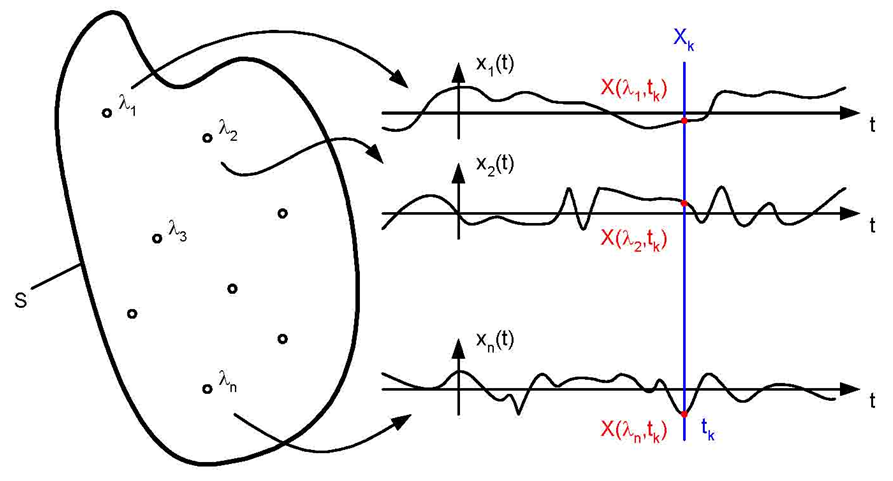
\includegraphics[width=10cm]{../NaT2/bilder/07_zufallsprozess.png}
\end{minipage}
\begin{minipage}{8.5cm}
	Bei einem \textbf{Zufallsprozess} wird jedem \textbf{Ergebnis} \boldmath$\lambda$ aus 
	dem \textbf{Ergebnisraum} $S$ eine \textbf{deterministische} \textbf{Funktion} $x(\lambda, t)$
	\unboldmath zugewiesen. \\
	Zufallsprozesse beschreiben eine deterministische Zeitfunktion ausgelöst durch ein Ergebnis eines
	Zufallsexperiments. \\
	Zeitlich \textbf{zufällig ablaufende Funktionen} können ebenfalls als \textbf{deterministische} Funktionen 
	\textbf{aufgefasst} werden, bei denen der Beobachter nie weiss, welche Funktion $x_\lambda(t)$ konkret
	vorliegt.	\\ \\
	Zum Vergleich: Bei Zufallsvariablen wird jedem Elementarereignis eine Zahl zugewiesen. 
\end{minipage} 
\vspace{0.5cm} \\
Beispiele von Zufallsprozessen:
\begin{itemize}
  \item \textbf{Binäre Datenquelle:} Das auftreten einer $1$ oder $0$ (Ergebnis $\lambda$) ist
  zufällig, jedoch sind die dazugehörigen Pulsformen $x(\lambda_0, t)$ und $x(\lambda_1, t)$
  bekannt.
  \item \textbf{Ethernet-Paket:} Da die Paketlänge $1518$ Bytes beträgt ist der Ergebnisraum $S$
  endlich und beinhaltet alle möglichen Bitkombinationen der Länge von $1518$ Bytes. Das Auftreten
  der jeweiligen Bitfolgen ist zufällig, jedoch ist dann der zeitliche Verlauf der jeweiligen
  Pulsformen vorbestimmt.
  \item \textbf{Manchester-Puls mit Rauschen:} Am Empfänger ist den Bitpulsen \textbf{thermisches Rauschen}
  überlagert. Da man den zeitlichen Verlauf der Rauschspannung nicht vorhersagen kann, existiert
  eine \textbf{unendliche Anzahl Ergebnise} $\lambda$. \\
  Eine deterministische Berechnung des zeitlichen Verlaufs ist nicht möglich, jedoch kann man die
  \textbf{statistischen Eigenschaften} der Rauschquellen aufgrund des physikalischen Modells exakt berechnet
  werden.
\end{itemize}

\subsection{Statistische Mittelwerte (Scharmittel) \schaum{166-7.3.B}}
Die statistischen Mittelwerte sind eine Funktion der Zeit $t$, da es sich um Mittelwerte über das
Ensemble (ganzer Ergebnisraum) handelt. Hierbei werden alle deterministischen Funktionen zu einem
bestimmten Zeitpunkt $t$ gemittelt. 

\renewcommand{\arraystretch}{1.4}
\begin{tabular}[c]{ p{3.5cm}  p{14.5cm}  }
	\textbf{Erwartungswert}: 	&  $\mu_{X}(t) = E\left[X(t)\right] =
          \int\limits_{-\infty}^{+\infty} x \cdot f_{X}(x;t)\;dx$ \\
   	\textbf{Autokorrelation}: 	& 	$R_{XX}(t_{1},t_{2}) = E\left[X(t_{1})X(t_{2})\right] =
          \int\limits_{-\infty}^{+\infty} \int\limits_{-\infty}^{+\infty} 
            x_{1} \cdot  x_{2}\cdot f_{X}(x_{1},x_{2};t_{1},t_{2})\;dx_{1} \;dx_{2}$ \\
	\textbf{Autokovarianz}:		&  $C_{XX}(t_{1},t_{2}) =
          E\left[ \left( X(t_{1})-\mu_{X}(t_{1})\right) \cdot
                  \left( X(t_{2})-\mu_{X}(t_{2})\right) \right] =
          R_{XX}(t_{1},t_{2}) - \mu_{X}(t_{1}) \cdot \mu_{X}(t_{2})$	
\end{tabular}
\renewcommand{\arraystretch}{1}

\subsection{Zeitliche Mittelwerte (Zeitmittel) \schaum{168-7.3.D}}
Hierbei werden die jeweiligen deterministischen Funktionen (Musterfunktionen) zeitlich gemittelt.
Wird das zeitliche Mittel über den gesamten Zufallsprozess berechnet, so handelt es sich bei den
zeitlichen Mittelwerten um \textbf{Zufallsvariablen}, d.h. die folgenden zwei Ausdrücke sind
abhängig davon (darum Index $_i$), welche Funktion genutzt wird.

%\renewcommand{\arraystretch}{1.4}
\begin{tabular}[c]{ p{4cm}  p{14.5cm}  }
	\textbf{Mittelwert}: 	&  
	$\overline{x_{i}} = \left\langle x_{i}(t) \right\rangle = 
           \lim\limits_{T \rightarrow \infty}
             \frac{1}{T} \int\limits_{-\frac{T}{2}}^{+\frac{T}{2}} x_{i}(t) \; dt$ \\
   	\textbf{Autokorrelation}: 	& 	
   	$\overline{R}_{X_{i}X_{i}}(\tau) = \left\langle x_{i}(t) \cdot x_{i}(t+\tau) \right\rangle = 
           \lim\limits_{T \rightarrow \infty}
             \frac{1}{T} \int\limits_{-\frac{T}{2}}^{+\frac{T}{2}} x_{i}(t) \cdot x_{i}(t + \tau) \; dt$\\
    \multicolumn{2}{l}{Falls der \textbf{Prozess stationär} ist gilt zudem: } \\
	\textbf{Mittelwert}: 	&  
	$E[\overline{x}] = 
           \lim\limits_{T \rightarrow \infty}
             \frac{1}{T} \int\limits_{-\frac{T}{2}}^{+\frac{T}{2}} E[x(t)] \; dt = 
             \frac{1}{T} \int\limits_{-\frac{T}{2}}^{+\frac{T}{2}} \mu_{X} \; dt = \mu_{X}(t)$  \\
   	\textbf{Autokorrelation}: 	& 	
   	$E[\overline{R}_{XX}(\tau)] = 
           \lim\limits_{T \rightarrow \infty}
             \frac{1}{T} \int\limits_{-\frac{T}{2}}^{+\frac{T}{2}} E[x(t)x(t+\tau)] \; dt =
             \frac{1}{T} \int\limits_{-\frac{T}{2}}^{+\frac{T}{2}} R_{XX}(\tau) \; dt = R_{XX}(\tau)$\\
\end{tabular}
\renewcommand{\arraystretch}{1}

\subsection{Stationarität \schaum{167-7.3.C}}
Ein stationärer Prozess verändert seine statistischen Eigenschaften über die
Zeit nicht. Wenn ein Prozess ergodisch ist, ist er auch stationär (nicht
umgekehrt).\\

\subsubsection{Streng Stationär (SSS - Strict Sense Stationary)}
% TODO genaue beschreibung streng, schwach stationär
Bei einem streng stationären Prozess bleiben die n-dimensionale WSK-Dichten über die
Zeit konstant. D.h. die \textbf{statistischen Eigenschaften} und somit auch die WSK-Dichten sind zu 
\textbf{allen Zeitpunkten dieselben}.
$$ f_X(x_1, x_2, \ldots, x_n; t_1, t_2, \ldots, t_n) =
		f_X(x_1, x_2, \ldots, x_n; t_1+c, t_2+c, \ldots, t_n+c) \qquad \forall (c,n \in
		\mathbb{R})$$
% Es gelten folgende Beziehungen: \\
% $$E[X(t)] = \mu_{X} \qquad \qquad
% R_{XX}(t_{1},t_{2}) = R_{XX}(\tau),\quad \text{ mit } \tau = t_{2} - t_{1} \qquad \qquad
% C_{XX}(t_{1},t_{2}) = R_{XX}(\tau) - \mu_{X}^{2}$$ 

\subsubsection{Schwach Stationär (WSS - Wide Sense Stationary) - Stationarität 2. Ordnung}
Bei einem schwach stationären Prozess sind die statistischen Eigenschaften zwar
\textbf{nicht zu jedem Zeitpunkt die selben}, jedoch sind sie \textbf{nicht} von einem \textbf{absoluten} Zeitpunkt, sondern
von der \textbf{Differenz} ($\tau$) \textbf{zweier Zeitpunkte} ($t_1, t_2$) abhängig.  \\ 
$$ f_X(x_1, x_2; t_1, t_2) = f_X(x_1, x_2; t_1+c, t_2+c) \qquad \forall (c \in
		\mathbb{R})$$
%Zudem gilt:\\
\renewcommand{\arraystretch}{1.4}
\begin{tabular}[c]{ |p{3.3cm}|  p{6.5cm} |p{8cm}| }
	\hline
	\textbf{Mittelwert}: 	&  $E[X(t)] = \mu_{X}(t) = \text{const.}$  
							& bleibt über die ganze Zeit konstant\\ 
	\hline
	\textbf{quad. Mittelwert}: 	&  $E[X^{2}(t)] = R_{XX}(0)$ &  \\ 
	\hline
	\textbf{Autokorrelation}: 	& 	$R_{XX}(t_{1},t_{2}) = R_{XX}(\tau)$
	& nur \textbf{abhängig} von der \textbf{Zeitdifferenz} $(\tau = t_2 - t_1)$ und \textbf{nicht direkt} von der \textbf{Zeit} $t$ \\
	 \hline
	 \textbf{Autokovarianz}:		& $ C_{XX}(t_{1},t_{2}) = R_{XX}(\tau) - \mu_{X}(t)^{2} = C_{XX}(\tau)$ & \\
	 \hline
\end{tabular}
\renewcommand{\arraystretch}{1}
 
Bei einem Zufallsprozess handelt es sich immer um ein WSS-Prozess, sobald der Erwartungswert
für jede Zeit $t$ konstant bleibt und die Autokorrelationsfunktion nur eine Funktion von $\tau$ ist,
d.h. beide statistischen Kennwerte bzgl. einer zeitlichen Verschiebung unabhängig sind.    
Jeder streng stationäre Prozess ist auch schwach stationär, aber nicht umgekehrt. 
        
%   \item Zwei Zufallsprozesse heissen Verbund-schwach-station\"ar, wenn jeder Prozess f\"ur sich 
%         schwach-station\"ar ist und zudem gilt:  
%         \begin{itemize}
%           \item[$\circ$] $R_{XY}(t_{1},t+\tau) = E[X(t)Y(t+\tau)] = R_{XY}(\tau)$ 
%         \end{itemize} 
%   \item Dann gilt auch:
%   \begin{itemize}
%      \item[$\circ$] $C_{XY}(\tau) = R_{XY}(\tau) - \mu_{X} \mu_{Y}$
%   \end{itemize} 
% \end{itemize} 

%TODO verbund schwach stationär

\subsection{Ergodizität \schaum{168-7.3.D}}
Ein stationärer Prozess ist zudem noch ergodisch, wenn \textbf{\textcolor{red}{alle} zeitlichen
Mittelwerten} (Zeitmittelwert und zeitlich gemittelte Autokorrelation) den \textbf{statistischen
Mittelwerten} (Erwartungswert und statistisch gemittelte Autokorrelation)
\textbf{entsprechen}. Jeder ergodische Zufallsprozess ist auch stationär, aber
nicht umgekehrt.
%\hspace{2cm} \textbf{Zeitmittel = Scharmittel}\\


	\begin{minipage}{5cm}
		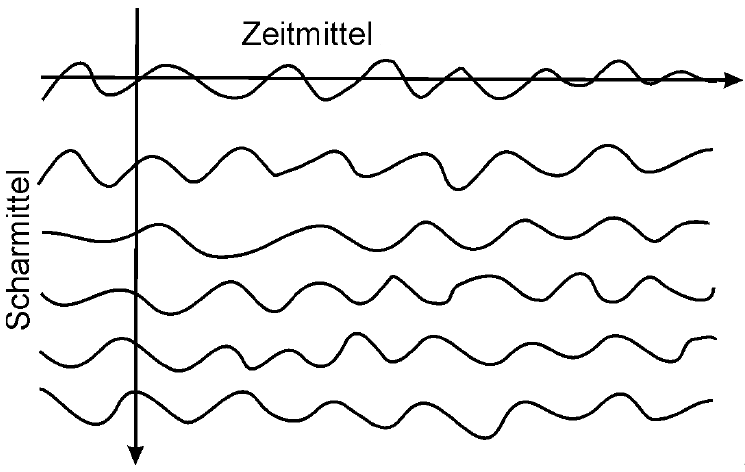
\includegraphics[width=4.7cm]{../NaT2/bilder/07_zeit-scharmittel.png}
  	\end{minipage}
	\begin{minipage}{13.5cm}
	\begin{tabular}{llll}  
    	Statistische MW $ \left\{
    	\begin{array}{ccc}
       		E[X(t)] & = & \overline{x}_i \\
       		R_{XX}(\tau) & = & \overline{R}_{X_iX_i}(\tau)
       \end{array}
		\right\} $
		Zeitliche MW (\textbf{const. für alle i})
    \end{tabular} \\

	\begin{tabular}{ll}
  		\multicolumn{2}{l}{Nur bei ergodischen Prozessen gilt zwingend:} \\
      $E[X(t)] = \overline{x} = \left\langle x(t) \right\rangle$ & DC-Level \\
      $E[X(t)]^{2} = (\overline{x})^{2} = \left\langle x(t) \right\rangle^{2}$ & DC-Leistung \\
      $E[X^{2}(t)] = R_{XX}(0) = \overline{x^{2}} = 
                     \left\langle x^{2}(t) \right\rangle $ & Gesamtleistung \\
      $\sigma_{X}^{2}(t) = \left\langle x^{2}(t) \right\rangle 
                           - \left\langle x(t) \right\rangle^{2}$ & AC-Leistung \\
      $\sigma_{X}(t) = \overline{\sigma}_{X}$ & RMS-Level (Effektivwert) des AC-Signals\\
    \end{tabular}
  	\end{minipage}


\subsection{Vergleich Stationär - Ergodisch}
\subsubsection{Mückenschwarm}
\textbf{Ergodisch:} Fliegen alle Mücken zusammen in einem Schwarm, so fliegt jede Mücke über die
ganze Zeit gemittelt (Zeitmittel) so schnell wie der ganze Schwarm im Mitel (Scharmittel), ansonsten
würde der Schwarm nicht zusammenhalten können. \\
\textbf{Stationär:} Ist eine Mücke krank und kann mit dem Schwarm nicht mithalten, so fliegt sie
alleine und v.a. langsamer. Somit ist ihre Durchschnittsgeschwindigkeit (Zeitmittel) nicht gleich
derjenigen des Schwarms (Scharmittel), also kommt sie später am Ziel an. \\
\textbf{Weder noch:} Fliegen die Mücken nach dem Start immer langsamer, so ist die
durchschnittliche Geschwindigkeit des Schwarms (Scharmittel) nicht konstant.

\subsubsection{Schulnoten}
\textbf{Ergodisch:} Alle Schüler müssten dieselbe Zeugnisnote (Zeitmittel) haben und zudem müsste
diese Note jeweils auch dem Klassenschnitt (Scharmittel) der einzelnen Prüfungen entsprechen. \\
\textbf{Stationär:} Der Klassenschnitt (Scharmittel) ist bei jeder Prüfung gleich, jedoch gibt es
unterschiedlich starke Schüler mit unterschiedlichen Zeugnisnoten (Zeitmittel). \\
\textbf{Weder noch:} Der Klassenschnitt (Scharmittel) ist immer unterschiedlich.

\subsubsection{Thermisches Widerstandsrauschen} 
Dies ist bei gleichbleibender Temperatur \textbf{ergodisch}.


\subsection{Korrelationen und Leistungsspektren \schaum{169-7.4}}
Formeln in diesem Abschnitt gelten für \textbf{stationäre} Prozesse. \\

\renewcommand{\arraystretch}{1.6}
\begin{tabular}[c]{|p{4cm}|p{6cm}|p{7.5cm}|}
	\hline
	\textbf{Autokorrelation}: 	&
		$R_{XX}(\tau) = E[X(t)X(t+\tau)]$\newline
  		$R_{XX}(\tau) \! \mid \leq R_{XX}(0) = E[X^{2}(t)]$ 
		&$R_{XX}(-\tau) = R_{XX}(\tau) \quad$ (gerade)\\
	\hline
  	\textbf{Kreuzkorrelation}: 	& 	
 		$R_{XY}(\tau) = E[X(t)Y(t+\tau)]$  
		& $R_{XY}(-\tau) = R_{YX}(\tau) \quad$ (Reihenfolge Indizes!) \\
		& $|R_{XY}(\tau)| \leq \frac{1}{2} \left[ R_{XX}(0)+R_{YY}(0)\right] $
		& $|R_{XY}(\tau)|  \leq \sqrt{R_{XX}(0)R_{YY}(0)}$ \\
	\hline
  	\textbf{Autokovarianz}: 	&  
		\multicolumn{2}{l|}{$C_{XX}(\tau) = E\!\left[ \left( X(t)      - E[X(t)]      \right) \cdot
    	\left( X(t+\tau) - E[X(t+\tau)] \right) \right] =
   		R_{XX}(\tau) - \mu^{2}_{X} $} \\
   	\hline
  	\textbf{Kreuzkovarianz}: 	& 	
   		\multicolumn{2}{l|}{$C_{XY}(\tau) = E\!\left[ \left( X(t)      - E[X(t)]      \right) \cdot
        \left( Y(t+\tau) - E[Y(t+\tau)] \right) \right] = R_{XY}(\tau) - \mu_{X}\mu_{Y} $}\\
  	  	& \multicolumn{2}{l|}{Zufallsprozesse bezeichnet man als zueinander \textbf{unkorreliert}, wenn $C_{XY}(\tau)0$}\\
   	\hline
\end{tabular}
\renewcommand{\arraystretch}{1}

\subsubsection{Spektrale Leistung \schaum{170-7.4.E,F}}
Autokorrelationsfunktion $R_{XX}(\tau)$ und Leistungsspektraldichte $S_{XX}(\omega)$ bilden ein
Fourier-\textbf{Transformationspaar}. \\ Die Leistungsspektraldichte kann als \textbf{mittlere Leistung pro Frequenzband }aufgefasst werden, sie ist
wie folgt definiert:                             
        $$ E\left[ \lim\limits_{T \rightarrow \infty} \frac{1}{T} \cdot \mid\!
        X(\omega) \!\mid^{2}\right] = \int\limits_{-\infty}^{+\infty}
        R_{XX}(\tau) \cdot e^{-j\omega\tau} \; d\tau = \boxed{S_{XX}(\omega)
        \qquad \IFT \qquad R_{XX}(\tau)} = \frac{1}{2\pi}
        \int\limits_{-\infty}^{+\infty}S_{XX}(\omega) \cdot e^{j\omega\tau} \;
        d\omega$$ $S_{XX}(\omega)$ ist rein reell und $\geq 0$. \\
Kreuzkorrelationen ($R_{YX}(\tau), R_{XY}(\tau)$) und Kreuz-Spektraldichten ($S_{YX}(\tau),
S_{XY}(\tau)$) bilden ein Fourier-Transformationspaar.
\begin{center}
	$R_{YX}(\tau) \FT S_{YX}(\omega) \qquad \qquad R_{XY}(\tau) \FT S_{XY}(\omega)$
\end{center}



\subsection{Übertragung von Zufallsprozessen durch LTI-Systeme \schaum{171-7.5}}
Ein Zufallsprozess wird durch ein LTI-System übertragen. \hspace{2cm} $Y(t) = L[X(t)] \Rightarrow
Y(t) = h(t) \ast X(t)$ \vspace{0.3cm}\\
\renewcommand{\arraystretch}{1.4}
 \begin{tabular}[c]{|p{2cm}| p{8.5cm} |p{8cm}| }
 	\hline
		&\textbf{Allgemein}
		& \textbf{WSS-Prozess} \\
	\hline
	\textbf{Mittelwert}
		& $E(Y(t)) = h(t) \ast E(X(t))$
		& $E(Y) = H(0) \cdot E(X)$ \\
	\hline
	\textbf{Auto-korrelation\textcolor{red}{*}}
		& {$R_{YY}(t_{1},t_{2}) = \int\limits_{-\infty}^{+\infty}
		\int\limits_{-\infty}^{+\infty} h(\alpha) h(\beta)
                      R_{XX}(t_{1}-\alpha, t_{2}-\beta) \; d\alpha \; d\beta$}
		& {$R_{YY}(\tau) = \int\limits_{-\infty}^{+\infty}
		\int\limits_{-\infty}^{+\infty} h(\alpha) h(\beta)
                      R_{XX}(\tau+\alpha-\beta) \; d\alpha \; d\beta$} \\
    \hline
	\textbf{Spektrale Leistung}
		&
		& $S_{YY}(\omega)= H^{\ast}(\omega) H(\omega) S_{XX}(\omega)
			= |H(\omega)|^{2} S_{XX}(\omega)$  \\
	\hline
\end{tabular}
\renewcommand{\arraystretch}{1} \\
\textcolor{red}{*} = Es ist viel einfacher die Autokorrelation aus der Spektralen Leistung
(Transformationspaar) - anstatt aus diesem höllischen Integral - auszurechnen. \\
Ein WSS-Prozess am Eingang erzeugt auch einen WSS-Prozess am Ausgang.

\subsection{Spezielle Zufallsprozesse \schaum{172-7.6}}
\subsubsection{Gauss'scher Zufallsprozess \schaum{172-7.6.A}}
Bein diesem Prozess ist die \textbf{Zufallsvariable} $X(t_{i})$ zu \textbf{jedem Zeitpunkt} $t_{i}$
\textbf{gaussverteilt}. Bsp.: thermisches Rauschen. \\
Zweidimensionaler Fall (gauss'sche Verbunddichte): 
       $$f_{XX}(x_{1},x_{2};t_{1},t_{2}) = \frac{1}{2\pi \sigma_{x_{1}}\sigma_{x_{2}}} \cdot
                                      e^{-\frac{(x_{1}-\mu_{x_{1}})^{2}}{2 \sigma^{2}_{x_{1}}}} \cdot
                                      e^{-\frac{(x_{2}-\mu_{x_{2}})^{2}}{2 \sigma^{2}_{x_{2}}}}$$ \\
Für unkorrelierte $X(t_{1})$ und $X(t_{2})$  ($C_{XX}(t_{1},t_{2})=0$) gilt:
        $$f_{XX}(x_{1},x_{2}; t_{1},t_{2}) = f_{X}(x_{1};t_{1}) \cdot f_{X}(x_{2};t_{2}) $$
$\mu_{X}(t)$ und $R_{XX}(t_{1}, t_{2})$ charakterisisieren einen gauss'schen Zufallsprozess
        vollst\"andig. \\
Ist ein gauss'scher Prozess WSS ist er zugleich auch SSS. Zudem ist wird ein gauss'scher
Zufallsprozess $X(t)$ am Ausgang eines LTI Systems $Y(t)$ wiederum gaussisch.

\subsubsection{Weisses Rauschen  \schaum{173-7.6.B}}
\begin{center}
	\begin{minipage}{8cm}
		$S_{XX}(\omega) = \dfrac{\eta}{2} \qquad R_{XX}(\tau) = \dfrac{\eta}{2} \cdot \delta(\tau)$ \\ \\
		Beispiel: therm. Rauschen von Widerständen \\
		\textbf{Nimmt} in der Praxis im \textbf{Tera-Hz Bereich ab}!
  	\end{minipage}
	\begin{minipage}{10cm}
		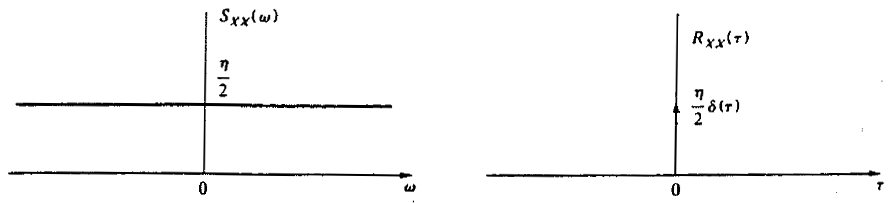
\includegraphics[width=9cm]{../NaT2/bilder/07_weisses_rauschen.png}
  	\end{minipage}
\end{center}

\subsubsection{Farbige Rauschsignale}
\renewcommand{\arraystretch}{2}
\begin{tabular}[c]{ | p{4cm} | p{3.5cm} | p{3cm} | p{6cm} | }
% 	\hline
% 		Weisses Rauschen
% 		& White Noise
% 		& $S_{XX}(\omega) = \dfrac{\eta}{2}$
% 		& \\
	\hline
		\textbf{Bezeichnung (De)}
		& \textbf{Bezeichnung (En)}
		& \textbf{Leist.-Spektrum}
		& \textbf{Anmerkung} \\
	\hline
		Rosa Rauschen
		& Pink Noise
		& $S_{XX}(\omega) = c \cdot \dfrac{1}{\omega}$
		& Testsignal für Tontechnik, wegen konstanter Leistung pro Oktave \\
	\hline
		Braunes/Rotes Rauschen
		& Brown/Red Noise
		&	$S_{XX}(\omega) = c \cdot \dfrac{1}{\omega^2}$
		& \\
	\hline
		Blaues Rauschen
		& Blue Noise
		&	$S_{XX}(\omega) = c \cdot \omega$
		& \\
	\hline
		Violettes Rauschen
		& Purple/Violet Noise
		&	$S_{XX}(\omega) = c \cdot \omega^2$
		& Bsp.: FM Demodulator Noise\\
    \hline
\end{tabular}
\renewcommand{\arraystretch}{1}

\subsubsection{Bandbeschränktes Rauschen \schaum{174-7.6.C}}
\begin{center}
	\begin{minipage}{8cm}
		$S_{XX}(\omega) = \begin{cases}
                      \dfrac{\eta}{2} & |\omega| \leq \omega_B \\
                      0 & |\omega| > \omega_B
                      \end{cases} \\ \\
		R_{XX}(\tau) =  \frac{1}{2\pi} \int\limits_{-\omega_{b}}^{+\omega_{b}}
                                           \frac{\eta}{2}  \cdot e^{j\omega\tau}\; d\tau
                      = \frac{\eta\omega_{B}}{2\pi} \frac{\sin(\omega_{B}\tau)}{\omega_{B}\tau}$
  	\end{minipage}
	\begin{minipage}{10cm}
		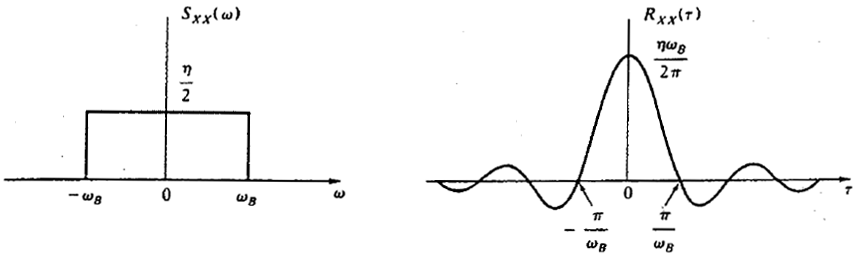
\includegraphics[width=9cm]{../NaT2/bilder/07_bandlimited_whitenoise.png}
  	\end{minipage}
\end{center}

\subsubsection{Schmalbandiger Zufallsprozess \schaum{174-7.6.D}}
\label{schmalbandiger_zufallsprozess}
	\begin{minipage}{9.5cm}
		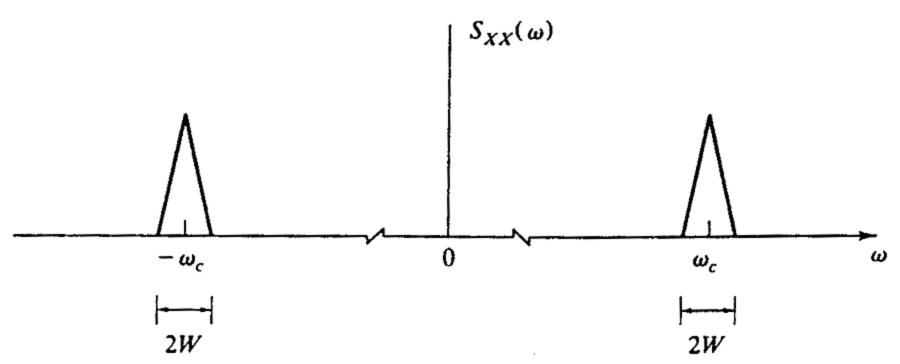
\includegraphics[width=9cm]{../NaT2/bilder/07_schmalbandiger_zufallsprozess.png}
  	\end{minipage}
	\begin{minipage}{8.8cm}
		Hierbei handelt es sich um einen WSS-Prozess mit \textbf{sehr kleiner Bandbreite} $2W$ verglichen mit der
		Mittenfrequenz $\omega_c$. \\
		Dies ist beispielsweise der Fall wenn \textbf{thermisches Widerstandrauschen} durch ein schmalbandiges
		Bandpass gefiltert wird. \\
		Im \textbf{Zeitbereich} manifestiert sich diese Funktion als \textbf{sinusförmiges} Signal mit
		zufälliger Amplitude und Phase. \\
		Bei $X_{c}(t)$ und $X_{s}(t)$ handelt es sich damit um bandbeschr\"anktes Rauschen im Basisband.
  	\end{minipage} \\
	\begin{minipage}{10cm}
		\boldmath$$X(t) = V(t) \cdot \cos \left[ \omega_{c}t + \phi(t) \right]$$ \unboldmath
		$$X(t) = X_{c}(t)\cos\omega_{c}(t) - X_{s}(t)\sin\omega_{c}(t)$$
		$$X_{c}(t) = V(t)\cos\phi(t) \qquad X_{s}(t) = V(t)\sin\phi(t)$$
		$$V(t) = \sqrt{X^{2}_{c}(t) + X^{2}_{s}(t)} \qquad \phi(t) = \arctan \frac{X_{s}(t)}{X_{c}(t)}$$
  	\end{minipage}
	\begin{minipage}{8cm}
		$V(t)$ Enveloppen-Funktion \\ 
        $\phi(t)$ Phasenfunktion. \\
		$X_{c}(t)$ gleichphasiger Anteil \\ 
        $X_{s}(t)$ Quadratur-Anteil        
  	\end{minipage} \\

Eigenschaften von $X_{c}(t)$ und $X_{s}(t)$: \\

\renewcommand{\arraystretch}{1.5}
\begin{tabular}{p{4.5cm} p{4.5cm} p{9cm}}
	$\mu_{X_{c}} = \mu_{X_{s}} = \mu_{X} = 0$
		& $\sigma^{2}_{X_{c}} = \sigma^{2}_{X_{s}} = \sigma^{2}_{X}$
		& $E\left[ X_{c}(t)X_{s}(t) \right]  = 0$ (unkorreliert \& orthogonal) \\
	\multicolumn{3}{c}{$S_{X_{c}X_{c}}(\omega) = S_{X_{s}X_{s}}(\omega)
                   = \left\lbrace
                       \begin{array}{ll}
                         S_{XX}(\omega -\omega_{c}) +S_{XX}(\omega +\omega_{c})
                                        & \mid\!\omega\!\mid \leq W \\
                         0              & \mid\!\omega\!\mid > W \\
                       \end{array} \right. $} \\ 
\end{tabular}
\renewcommand{\arraystretch}{1}

Ist $X(t)$ ein Gauss-Prozess, sind auch $X_{c}(t)$ und $X_{s}(t)$ gaussisch. Dann ist $V(t)$
Rayleigh-verteilt zu jedem Zeitpunkt t und $\Phi(t)$ gleichverteilt ($0..2\pi$) zu jedem
Zeitpunkt t. 

\newpage
\section{Rauschen in analogen Kommunikationssystemen \schaum{202-8}}
\textbf{Rauschen} \textbf{verschlechtert} die \textbf{Performance}. Bei \textbf{analogen} Systemen
macht sich dies beim \textbf{Signal-Rausch-Abstand (SNR)} bemerkbar.
\subsection{Gemeinsame Charakteristik: gauss'scher Kanal}
\begin{figure}[!ht]
\begin{center}
	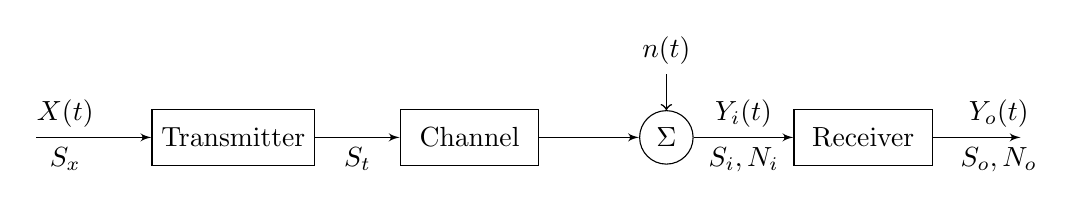
\begin{tikzpicture}[>=latex']
    \node[input, name=input] {};
    \node[block, right of=input, name=transmitter] {Transmitter};
    \node[block, right of=transmitter, name=channel, node distance=3cm] {Channel};
    \node[sum, right of=channel, name=sum, pin={[pin style]above:$n(t)$}] {$\Sigma$};
    \node[block, right of=sum, name=receiver] {Receiver}; 
    \node[output, right of=receiver, name=output, node distance=2cm] {};        
    
    \draw[->] (input) -- (transmitter)
       node[above, near start] (Xt) {$X(t)$}
       node[below, near start] (Xt) {$S_x$};
    \draw[->] (transmitter) -- node[below] {$S_t$} (channel);
    \draw[->] (channel) -- (sum);
    \draw[->] (sum) -- (receiver)
       node[above, midway] {$Y_i(t)$}
       node[below, midway] {$S_i, N_i$};
    \draw[->] (receiver) -- (output)
       node[above, near end] {$Y_o(t)$}
       node[below, near end] {$S_o, N_o$};
\end{tikzpicture}    
\end{center}
\end{figure}

Die Voraussetzungen für eine einfache Berechnung mit Hilfe von diesem Modell (gauss'scher Kanal)
sind die folgenden:
\begin{itemize}
  \item $n(t)$ ist \textbf{mittelwertfreies} ($E[n] = 0$) gauss'sches Rauschen mit $S_{nn}(\omega) = \eta/2$
  \item $n(t)$ ist mit $X \left( t \right)$ \textbf{unkorreliert} $\left( Cov
  \left(X,n \right) = E \left[ X \cdot n \right] - E \left[ X \right] \cdot E
  \left[ n \right] = 0 \right) \quad \rightarrow \quad E[X\cdot n] = 0$
\end{itemize}
Somit gilt: $ \qquad E[Y_o^2]= E[(X_o + n_o)^2] = E[X_0^2] + \underbrace{E[2 \cdot X_o \cdot n_o]}_0 + E[n_o^2] = S_o + N_o
\quad \text{ und } \quad SNR_o = \left(\dfrac{S}{N}\right)_o = \dfrac{E[X_o(t)^2]}{E[n_o(t)^2]}$ \\ \\
Weist der Kanal eine \textbf{Dämpfung} $A_{db}$ auf, so muss diese bei den Berechnungen berücksichtigt
werden: $S_{i_{dB}} = S_{t_{dB}} - A_{dB}$



\subsection{Referenzmodell: Basisband \schaum{203-8.3}}
Die Berechnungen im Basisband gelten als \textbf{Referenz}, für den \textbf{Vergleich} mit
\textbf{anderen Systemen}. \\

\begin{figure}[!ht]
\begin{center}
	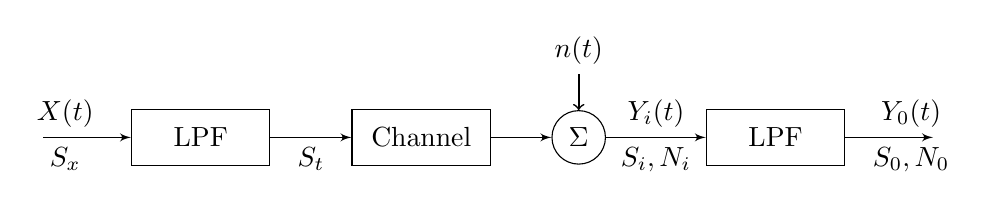
\begin{tikzpicture}[>=latex']
    \node[input, name=input] {};
    \node[block, right of=input, name=lpf1, node distance=2cm] {LPF};
    \node[block, right of=lpf1, name=channel, node distance=2.8cm] {Channel};
    \node[sum, right of=channel, name=sum, pin={[pin style]above:$n(t)$}, node distance = 2cm] {$\Sigma$};
    \node[block, right of=sum, name=lpf2] {LPF}; 
    \node[output, right of=lpf2, name=output, node distance=2cm] {};        
    
    \draw[->] (input) -- (lpf1)
       node[above, near start] {$X(t)$}
       node[below, near start] {$S_x$} ;
    \draw[->] (lpf1) -- node[below] {$S_t$} (channel);
    \draw[->] (channel) -- (sum);
    \draw[->] (sum) -- (lpf2)
       node[above, midway] {$Y_i(t)$}
       node[below, midway] {$S_i, N_i$};
    \draw[->] (lpf2) -- (output)
       node[above, near end] {$Y_0(t)$}
       node[below, near end] {$S_0, N_0$};
\end{tikzpicture}
\end{center}
\end{figure}

Wiederum müssen ebenfalls gewisse Einschränkungen gemacht werden für eine einfachere Berechnung:\\
\begin{tabular}{l l}
  $\bullet$ $X(t)$ ist mittelwertfrei: & $E[X]=0$ \\
  $\bullet$ $X(t)$ ist stationär und ergodisch: & $<x_{\lambda}(t)> = E[X] = 0 \quad (\text{für alle } x_{\lambda}(t))$\\
  $\bullet$ $X(t)$ ist bandbeschränkt: & $S_{XX}(\omega) = 0 $ für $\omega > W$ durch den idealen Tiefpassfilter
  mit Bandbreite $W = 2 \pi B$\\
  $\bullet$ Der Kanal ist verzerrungsfrei : 
  & $X_o(t) = X(t-t_d)$\\ 
  & \\
  Signalleistung am Ausgang des Empf.: 
  & $S_o = E[X_o^2(t)] = E[X^2(t-t_d)] = \frac{1}{2\pi}\int\limits_{-W}^{+W}S_{XX}(\omega)d\omega = S_X = S_i$\\
  Rauschleistung am Ausgang des Empf.: 
  & $N_o = E[n_o^2(t)] = \frac{1}{2\pi}\int\limits_{-W}^{+W}S{nn}(\omega) \;d\omega  = \frac{1}{2\pi}\int\limits_{-W}^{+W}\frac{1}{2/pi}\; d\omega = \eta \frac{W}{2\pi} = \eta B$\\
  
\end{tabular}

$$ \text{Die Rauschleistung im Basisband: } \qquad \boxed{\left(\dfrac{S}{N}\right)_o =
\dfrac{S_o}{N_o} = \dfrac{S_i}{\eta B} = \gamma} \qquad \text{dient zum Vergleich mit anderen
Systemen.}$$

\subsubsection{Equalizer als LPF}
Neben einem idealen LPF kann auch ein Equalizer (z.B. RC-Filter) eingesetzt werden. Dabei gilt:\\
\textbf{Allgemein:} $N_{o_{eq}} = \frac{1}{2\pi}\int\limits_{-\infty}^{+\infty} \underbrace{\frac{\eta}{2}}_{S_{nn}(\omega)}\cdot|H_{eq}(\omega)|^2 \cdot d\omega$  \hspace{1cm}
\textbf{RC-Filter} mit $H_{eq} = H_{RC} = \frac{1}{1+j\frac{\omega}{2\pi f_c}} \Rightarrow N{o_{RC}} = \eta\cdot f_c \cdot \frac{\pi}{2}$ 

\subsection{Amplitudenmodulation \schaum{204-8.4}}
\begin{figure}[!ht]
\begin{center}
	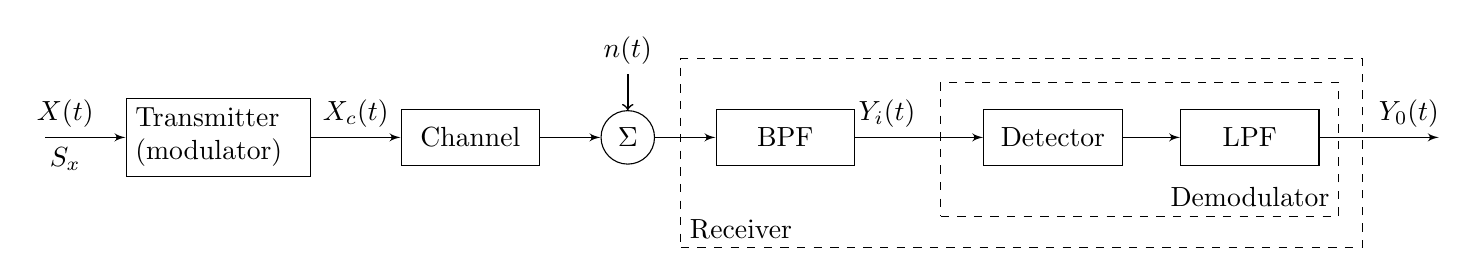
\begin{tikzpicture}[>=latex']
    \node[input, name=input] {};
    \node[block, right of=input, name=transmitter, node distance=2.2cm, text width=6em] {Transmitter (modulator)};
    \node[block, right of=transmitter, name=channel, node distance=3.2cm] {Channel};
    \node[sum, right of=channel, name=sum, pin={[pin style]above:$n(t)$}, node distance = 2cm] {$\Sigma$};
    \node[block, right of=sum, name=bpf, node distance = 2cm] {BPF};
    \node[block, right of=bpf, name=detector, node distance=3.4cm] {Detector};
    \node[block, right of=detector, name=lpf] {LPF};
    \node[output, right of=lpf, name=output, node distance=2.4cm] {};        
    
    \draw[->] (input) -- (transmitter)
       node[above, near start] {$X(t)$}
       node[below, near start] {$S_x$} ;
    \draw[->] (transmitter) -- node[above] {$X_c(t)$} (channel);
    \draw[->] (channel) -- (sum);
    \draw[->] (sum) -- (bpf);
    \draw[->] (bpf) -- node[above, near start] {$Y_i(t)$} (detector);
    \draw[->] (detector) -- (lpf);
    \draw[->] (lpf) -- (output)
       node[above, near end] {$Y_0(t)$};
    
    %% Rechtecke
    \node at ($(detector.south west)-(0.3cm,0.4cm)$) (demo_SW) {};
    \node at ($(lpf.north east)+(0,0.1cm)$) (demo_NE) {};
    \node[draw=black, rectangle, dashed, fit=(demo_SW) (demo_NE)] (demodulator) {};
    \node[anchor=south east] at (demodulator.south east) {Demodulator};
    
    \node at ($(bpf.south west)-(0.2cm,0.8cm)$) (rec_SW) {};
    \node at ($(lpf.north east)+(0.3cm,0.4cm)$) (rec_NE) {};
    \node[draw=black, rectangle, dashed, fit=(rec_SW) (rec_NE)] (receiver) {};
    \node[anchor=south west] at (receiver.south west) {Receiver};
\end{tikzpicture}
\end{center}
\end{figure}
Das Rauschsignal am Eingang des Demodulators ist wie folgt definiert
\verweis{schmalbandiger_zufallsprozess}{Schmalbandiger Zufallsprozess}:  

	$$ Y_i(t) = X_c(t) + n_i(t)$$
	$$n_i(t) = n_c(t) \cos(\omega_c t) - n_s(t) \sin(\omega_c t) $$
	$$ E[n_c^2(t)] = E[n_s^2(t)] = E[n_i^2(t)] = 2 \eta B \quad \text{und} \quad E[n_c\cdot n_s] = 0$$



\subsubsection{DSB-SC, (SSB) \schaum{205-8.4.A.1,2}}
\textbf{DSB-SC mit synchronem Detektor}\\
\begin{minipage}{7.5cm}
	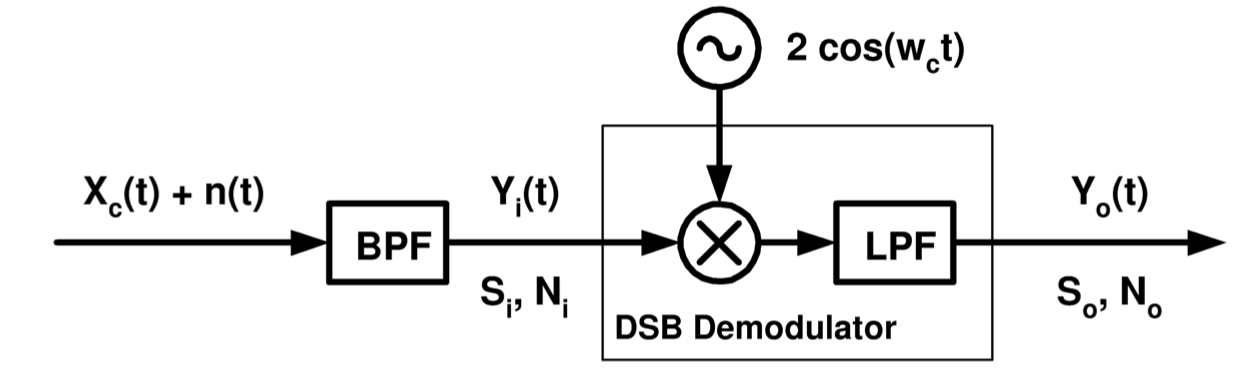
\includegraphics[width = 7cm]{./bilder/08_Sync_Detektor_DSB}
\end{minipage}
\begin{minipage}{11cm}
  $\bullet$ Am Eingang des Demodulators:\\ 
  \hspace*{0.3cm}$Y_i(t) = A_c X(t) \cos (\omega_c t) + n_i(t) = [A_c X(t) + n_c(t)]\cos(\omega_c t) - n_s(t)\sin(\omega_c t)$\\
  $\bullet$ Am Ausgang des Demodulator:\\ 
  \hspace*{0.3cm} $Y_o(t) = A_c X(t) + n_c(t) = X_o(t) + n_o(t)$
\end{minipage}\\ \\
Ein Mass für die Effizienz des Demodulators ist der sogenannte Detektor-Gewinn: \\
$$ \alpha_{d_{DSB-SC}} = \dfrac{\text{SNR}_{out}}{\text{SNR}_{in}} = 2 \approx 3 dB
\qquad \qquad
 \alpha_{d_{SSB}} = \dfrac{\text{SNR}_{out}}{\text{SNR}_{in}} = 1
$$
Ein DSB-SC Demodulator verbessert also die SNR zwischen Ein- und Ausgang um Faktor 2, bei SSB
bleibt die SNR gleich. Da SSB jedoch nur die halbe Bandbreite von DSB-SC besitzt, ist auch die
Eingangs-Rauschleistung bei SSB halb so gross wie bei DSB-SC. \\
Somit haben im Endeffekt SSB und DSB-SC \textbf{dieselbe Rausch-Performance} wie ein Basisbandsignal: 
	$$ \left(\dfrac{S}{N}\right)_0 =
	\dfrac{A_c^2 S_x}{2 \eta B} = \dfrac{\frac12 A_c^2 S_x}{\eta B} = \dfrac{S_i}{\eta B} = \gamma $$

\subsubsection{Gewöhnliche AM \schaum{206-8.4.A.3}}

\textbf{Synchroner Detektor}\\
\begin{minipage}{7.5cm}
	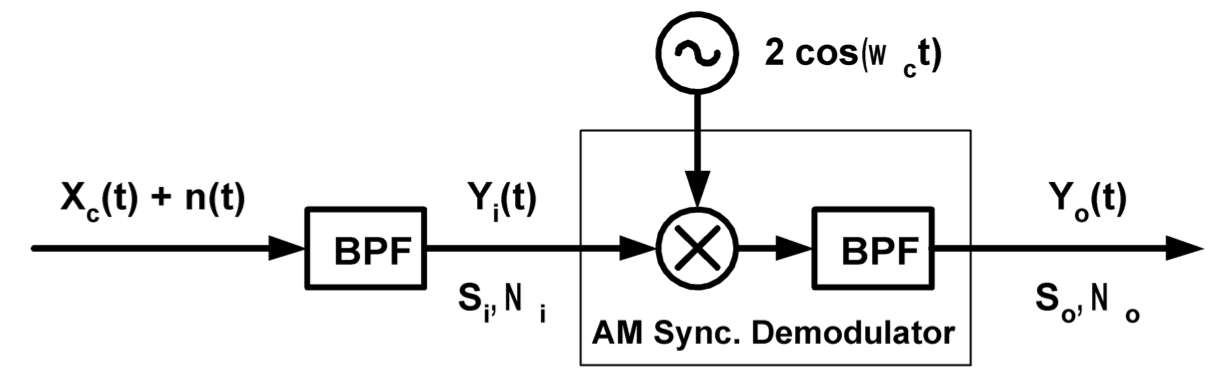
\includegraphics[width = 7cm]{./bilder/08_Sync_Detektor_AM}
\end{minipage}
\begin{minipage}{11cm}
  $\bullet$ Am Eingang des Demodulators:\\ 
  \hspace*{0.3cm}$Y_i(t) = A_c(1 + \mu X(t)) \cos (\omega_c t) + n_i(t)$ \qquad mit $\mu \leq 1$ und $X(t) \leq 1$\\
  $\bullet$ Am Ausgang des Demodulator:\\ 
  \hspace*{0.3cm} $Y_o(t) = A_c\mu X(t) + n_c(t) = X_o(t) + n_o(t)$
\end{minipage}\\ \\

$$ \left(\dfrac{S}{N}\right)_0 =
\dfrac{\mu^2 S_x}{1 + \mu^2 S_x} \left(\dfrac{S_i}{\eta B}\right) = \dfrac{\mu^2 S_x}{1 + \mu^2
S_x} \gamma \underbrace{\leq \dfrac{\gamma}{2}}_{\text{daher weniger geeignet als DSB-SC}} \qquad \qquad
\alpha_{d_{AM}} = \dfrac{2 \mu^2 S_x}{1 + \mu^2 S_x} \leq 1$$


\textbf{Enveloppe Detektor} \\
Für \boldmath$ \textbf{SNR}_i \gg 1 $ gelten dieselben Formeln wie beim \textbf{synchronen
Detektor}. \\ \\ Für \boldmath$ \textbf{SNR}_i \ll 1 $ lohnt es sich nicht solche
Berechnungen aufzustellen, da das demodulierte Signal \textbf{nicht mehr brauchbar} wird, weil das Rauschen so enorm dominiert. \\
Der \textbf{Übergang} zwischen \textbf{ausreichender} Übertragungsqualität und \textbf{unbrauchbarer}  
Übertragung beginnt ab \unboldmath$ \text{SNR}_{i_{dB}} \approx 10 \text{dB} $ und erfolgt
\textbf{sehr schnell}.

\subsection{Winkelmodulierte Systeme \schaum{208-8.5}}
\begin{minipage}{10cm}
	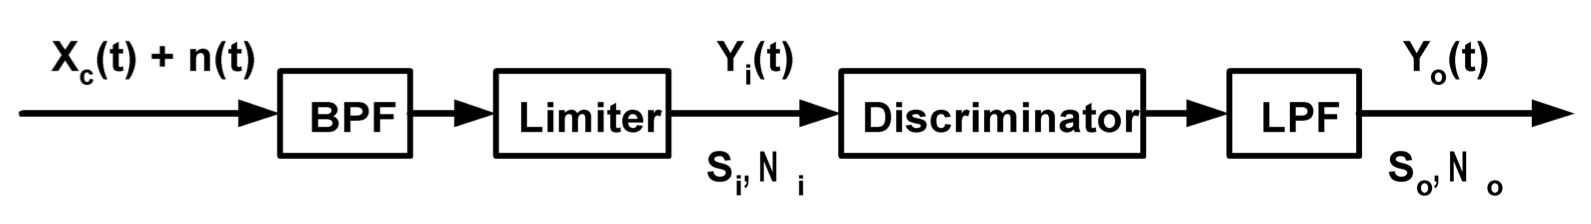
\includegraphics[height=1.3cm]{../NaT2/bilder/08_noise_anglemod.png}
\end{minipage}
\begin{minipage}{9cm}
	Signal am Eingang des Detektor:\\
	\hspace*{0.3cm} $Y_i(t) = A_c \cos(\omega_c t + \phi(t)) + n_i(t)$ \qquad mit \quad $S_i = \frac{1}{2} A_c^2$ \\
	\hspace*{0.6cm} \textbf{PM:} \quad $\phi = k_p X(t)$\\
	\hspace*{0.6cm} \textbf{FM:} \quad $\phi = k_f \int\limits_{-\infty}^{t} X(\tau) \; d\tau$ \\
	Rauschen am Eingang des Detektors:\\ 
	\hspace*{0.3cm} $n_i(t) = \underbrace{v_n(t)}_{n-Ampl.} \cdot \cos(\omega_c t + \phi_n(t))$\quad mit \quad $N_i = 2 (D+1)B_m\cdot\eta$\\
	\hspace*{0.6cm} $D$: \quad Hubverhältnis $\Delta f / B_m = \Delta \omega / W_m$
\end{minipage}\\ \\
Der Limiter \textbf{limitiert} das Signal - somit auch das Rauschen - in der \textbf{Amplitude}, 
sodass das \textbf{Rauschen} nur noch in der \textbf{Phase enthalten} ist. 
Die \textbf{SNR} wird daher \textbf{nur durch }die \textbf{Phase beeinflusst}. \\ 

Für die Winkelmodulation ist der Träger-Rauschabstand (CNR - Carrier-to-Noise-Ratio) wichtig: 
CNR = $ \dfrac{A_c^2}{2 \eta B_T} = \left(\dfrac{S}{N}\right)_i$. \\
\textbf{Nur wenn} das \textbf{Signal dominant} ist (CNR $\gg 1$), können die unten aufgeführten
Formeln angewendet werden. \\ 
Im Falle von (CNR $\ll 1$) tritt ein ähnlicher Effekt auf wie bei AM (SNR $\ll 1$), 
sodass das demodulierte Signal nicht mehr brauchbar wird. Der \textbf{Übergang} zwischen \textbf{ausreichender} Übertragungsqualität und \textbf{unbrauchbarer}  
Übertragung beginnt bei kleiner Deviation ($D \approx 2$) ab einer \unboldmath$ \text{SNR}_{i}$ von $(C/N)_i \approx 10 \text{dB} $ und erfolgt \textbf{sehr schnell}. Bei grösserer Deviation D setzt der Schwellwert Effekt schon bei höherer $SNR_i$ ein.

\subsubsection{Ausgang bei PM $(C/N \gg 1)$ \schaum{210-8.5.B}}
$$ Y_o(t) = \theta(t) = k_p X(t) + \frac{n_s(t)}{A_c}$$ 
$$ \left(\dfrac{S}{N}\right)_0 =
\dfrac{k_p^2 A_c^2 S_x}{2 \eta B} = k_p^2 S_x \gamma $$

\subsubsection{Ausgang bei FM $(C/N \gg 1)$ \schaum{210-8.5.C}}
$$ Y_o(t) = \frac{d \theta (t)}{dt} = k_f X(t) + \frac{n_s'(t)}{A_c}$$
$$ \left(\dfrac{S}{N}\right)_0 =
3 \left(\dfrac{k_f^2 S_x}{W^2}\right) \left(\dfrac{Ac^2}{2 \eta B}\right)
= 3 \left(\frac{k_f^2 S_x}{W^2}\right) \gamma = 
3 \left(\dfrac{\Delta \omega}{W}\right)^2 S_x \gamma = 3 D^2 S_x \gamma$$ \\ \\

$$B_{FM} = 2(\Delta f + B_S) = 2(D+1)B_S \qquad mit \quad B_S = B_m + \underbrace{B_{LP}}_{\text{zusätzliche Bandbreite durch Rauschen}}$$

\begin{landscape}
\newpage
\subsection{Zusammenfassende Tabelle \tiny{(Freundlicherweise zur Verfügung gestellt von Herrn T.
Kneubuehler})}
\renewcommand{\arraystretch}{2.3}
\begin{tabular}{|c|c|c|c|c|c|c|}
  \hline
    & Baseband
    & DSB-SC (SSB)
    & AM Coherent
    & AM Envelope
    & PM
    & FM          \\
  \hline
  Nachrichtensignal
    & \multicolumn{6}{c|}
    {Zufallsprozess $X(t)$ mit $\left| X(t) \right| \leq 1$
     bzw. $\left| x_{\lambda}(t) \right| \leq 1$ f\"ur alle $\lambda$ des Ergebnisraums $S$} \\
  \hline
  Leistung $S_{X}$ von $X(t)$
    & \multicolumn{6}{c|}
      {$S_{X} = S_{X}(t) = E\left[ X^{2}(t)\right] \leq 1$,
      (weil $\left| X(t) \right| \leq 1$)}\\
  \hline
  Bandbreite von $X(t)$
    & \multicolumn{6}{c|}{B} \\
  \hline
  Eingangsnutzsignal $X_{i}(t)$
    & $X(t)$
    & $X(t) A_{c}\cos(\omega_{c}t)$
    & \multicolumn{2}{c|}{$A_{c}(1+\mu X(t))\cos(\omega_{c}t)$}
    & \multicolumn{1}{c|} {$A_{c}\cos(\omega_{c}t + k_{p}X(t))$}
    & {$A_{c}\cos(\omega_{c}t + k_{f}\int\limits_{-\infty}^{t} X(\tau)\;d\tau)$}  \\
  \hline
  Leistung $S_{i}$ von $X_{i}(t)$
    & $S_{X}$
    & $\dfrac{1}{2}A_{c}^{2} S_{X}$
    & \multicolumn{2}{c|}{$\dfrac{1}{2}A_{c}^{2} (1 + \mu^{2}S_{X}) $}
    & \multicolumn{1}{c|} {$\dfrac{1}{2}A_{c}^{2}$}
    & {$\dfrac{1}{2}A_{c}^{2}$} \\
  \hline
  Bandbreite von $X_{i}(t)$ ; $B_t$
    & $B$
    & $2B \text{ (SSB}: B)$
    & \multicolumn{2}{c|}{$2B$}
    & \multicolumn{1}{c|}{$2(D + 1) B$}
    & {$2(D + 1) B$} \\
  \hline
  Rauschleistung am Eingang $N_i$
    & $\eta B$
    & $2\eta B$
    & \multicolumn{2}{c|}{$2\eta B$}
    & \multicolumn{1}{c|}{$2(D + 1)\eta B$}
    & {$2(D + 1)\eta B$} \\
  \hline
  SNR am Eingang $\left(\dfrac{S}{N}\right)_{i}$
    & $\dfrac{S_{i}}{\eta B}$
    & $\dfrac{\dfrac{1}{2}A_{c}^{2} S_{X}}{2\eta B}$
    & \multicolumn{2}{c|}{$\dfrac{\dfrac{1}{2}A_{c}^{2} (1 + \mu^{2}S_{X})}{2\eta B}$}
    & \multicolumn{1}{c|}{$\dfrac{\dfrac{1}{2}A_{c}^{2}}{2(D + 1)\eta B}$}
    & {$\dfrac{\dfrac{1}{2}A_{c}^{2}}{2(D + 1)\eta B}$} \\
  \hline
  Ausgangsnutzsignal $X_{o}(t)$
    & $X(t)$
    & $A_{c}X(t)$
    & \multicolumn{2}{c|}{$A_{c}\mu X(t)$}
    & \multicolumn{1}{c|} {$k_{p}X(t)$}
    & {$k_{f}X(t)$}  \\
  \hline
  Leistung $S_{o}$ von $X_{o}(t)$
    & $S_{X}$
    & $A_{c}^{2} S_{X}$
    & \multicolumn{2}{c|}{$A_{c}^{2}\mu^{2}S_{X} = \frac{2\mu^2S_X}{1+\mu^2S_X}S_i$}
    & \multicolumn{1}{c|} {$k_{p}^{2}S_{X}$}
    & {$k_{f}^{2}S_{X}$} \\
  \hline
  Rauschleistung am Ausgang $N_0$
    & $\eta B$
    & $2\eta B$
    & \multicolumn{2}{c|}{$2\eta B$}
    & \multicolumn{1}{c|}{$\dfrac{1}{A_{c}^{2}/2} \eta B$}
    & {$\dfrac{1}{3}\dfrac{(2\pi B)^{2}}{A_{c}^{2}/2} \eta B$} \\
  \hline
  SNR am Ausgang $\left(\dfrac{S}{N}\right)_{o}$
    & $\dfrac{S_{i}}{\eta B}$
    & $\dfrac{A_{c}^{2} S_{X}}{2\eta B} = \dfrac{S_{i}}{\eta B}$
    & \multicolumn{2}{c|}{$\dfrac{A_{c}^{2}\mu^{2}S_{X}}{2\eta B}$}
    & \multicolumn{1}{c|}{$\dfrac{k_{p}^{2}A_{c}^{2}S_{X}}{2\eta B}$}
    & {$\dfrac{3 D^{2}A_{c}^{2}S_{X}}{2\eta B}$} \\
  \hline
  $\left(\dfrac{S}{N}\right)_{o}$ ausgedr\"uckt mit  $\gamma = \dfrac{S_{i}}{\eta B}$
    & $\gamma$
    & $\gamma$
    & \multicolumn{2}{c|}{$\dfrac{\mu^{2}S_{X}}{1 + \mu^{2}S_{X}}\gamma$}
    & \multicolumn{1}{c|}{$k_{p}^{2}S_{X}\gamma$}
    & {$3 D^{2}S_{X}\gamma$} \\
  \hline
\end{tabular}
\renewcommand{\arraystretch}{1}
\\[0.5cm]
\textbf{Wichtige Anmerkung}  \\
\begin{itemize}
  \item $S_X = (\frac{s_{pk}}{c})^2$
  \item Die Formeln der Tabelle gelten für dimensionslose, stationäre und mittelwertfreie Signale.
  \item Der Zufallsprozess liegt zudem in normierter Form vor, wie aus der Tabelle hervorgeht.
  \item Soll die SNR für konkrete physikalisch vorliegende Signale berechnet werden,
		müssen für die Amplituden und Leistungen am Eingang des Empfängers geeignete Saklierungsfaktoren
		verwendet werden.
  \item Handelt es sich beim Empfäger zudem um einen aktiven Schaltungsblock,
		ist das Signal (sowie der Rauschanteil) am Ausgang des Empfäangers ebenfalls mit den Parametern
		des Empfängers zu skalieren.
	\item $D=\frac{\Delta\omega}{W}=\frac{\Delta f}{B} = k_p = \frac{k_f}{W}$
\end{itemize}
\end{landscape}

\newpage
\section{Optimaler Detektor - Rauschen in digitalen Kommunikationssys. \formelbuch{227-9}}
\textbf{Rauschen} \textbf{verschlechtert} die \textbf{Performance}, bei \textbf{digitalen} Systemen zeigt sich dies in der
\textbf{Bitfehlerrate} $P_e$. \\
Diese Kapitel behandelt digitale Signale, welche über einen verzerrungsfreien Kanal gesendet werden
und mit einem Additiven Weissen Gauss'schen Rauschen (AWGN) versetzt werden. 

\skriptsubsection{Binäres Übertragungssystem}{226-9.2}
Ein \textbf{binäres Signal} $s_i(t)$ \verweiskurz{09_binary_signals_error} wird
über einen verzerrungsfreien Kanal gesendet. \\
\begin{center}
 	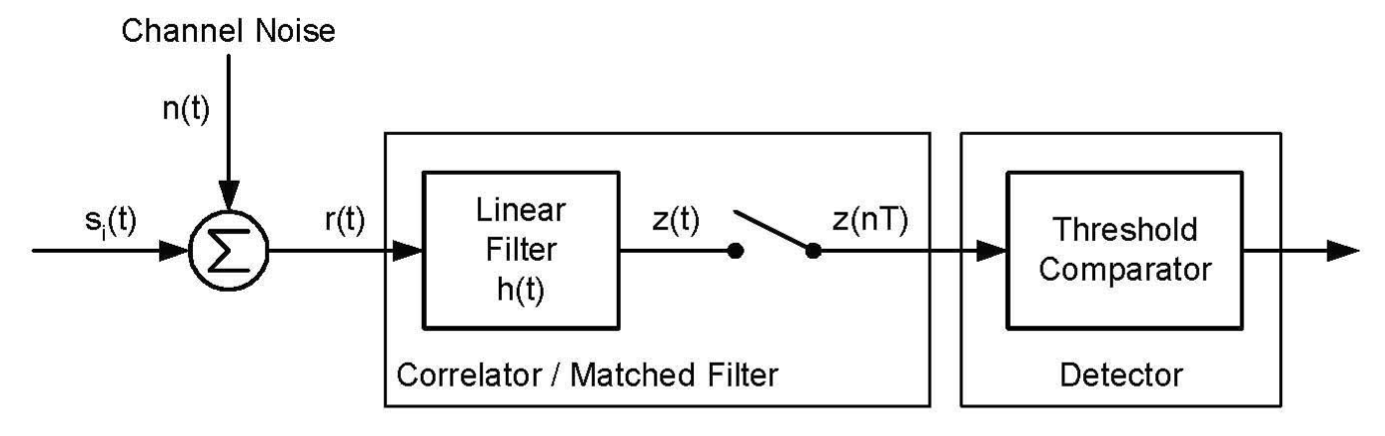
\includegraphics[height=3cm]{bilder/09_digital_signal_detection.png}
\end{center}

$$s_i(t) = \begin{cases}
          	s_1(t) & 0 \leq t \leq T \qquad \text{für Logisch } 1 \\
          	s_2(t) & 0 \leq t \leq T \qquad \text{für Logisch } 0          	
          \end{cases} 
				\qquad \overset{Rauschen}{\Longrightarrow} \qquad 
			r(t) = s_i(t) + n(t) 
				\qquad \overset{Filter}{\Longrightarrow} \qquad 
			z(t) = r(t) \ast h(t)$$ \\

\begin{enumerate}
  \item Am \textbf{Empfänger} $r(t)$ liegt das \textbf{Signal} $s(t)$ zusätlich mit einem Additiven 
  		Weissen Gauss'schen (AWGN) \textbf{Rauschen} $n(t)$ vor.
  \item Mit dem \textbf{linearen Filter} wird das Signal-Rausch-Verhältnis (\textbf{SNR})
		\textbf{optimiert} (so \textbf{gross} wie möglich gemacht). Das Signal nach dem Filter sollte
		möglichst \textbf{wenig Rauschen} aber \textbf{viel Signalanteil} enthalten. \\
		Hierbei können zwei Strategien angewendet werden, das Matched Filter 
		\verweiskurz{09_matched_filter} oder der Korrelator
		\verweiskurz{09_korrelator}.
  \item Anschliessend wird das Signal \textbf{zeitdiskretisiert}, also immer nach einer konstanten Zeit
  		(Samplingzeit $t = T$) abgetastet. Dadurch resultiert: $z(T) = a_i(T) + n_0(T)$, wobei $a_i(T)$
  		dem Signalanteil und $n_o(T)$ dem Rauschanteil entspricht. \\
  		Dies entspricht zwei Normalverteilungen, welche um die Mittelwerte ($a_1, a_2$) angeordnet sind.
  \item Schlussendlich wird mit dem Schwellwertdetektor entschieden, welches Signal
  		höchstwahrscheinlich gesendet wurde. Man unterscheidet die zwei verschiedenen Arten von
  		Detektoren: \\ \textbf{Hard-Decision:} Das Resultat des Detektors ist eine endgültige
  		Entscheidung (0 oder 1). Die Entscheidung wird mit Hilfe des Schwellwerts $\lambda_0$ gefällt.\\ 
  		\textbf{Soft-Decision:} Für 0 und 1 werden Wahrscheinlichkeiten bestimmt und verarbeitet.
\end{enumerate}

\subsection{Optimaler Detektor}
\skriptsubsubsection{Hypothesen und Fehlerwahrscheinlichkeit}{227-9.2,3.A}
	Für die Entscheidung existieren zwei \textbf{Hypothesen} ($H_1 \Rightarrow s_1$ wurde gesendet, 
	$H_2 \Rightarrow s_2$ wurde gesendet): \\ 
	Falls das gesamplete Signal ($z(T) > \lambda_0$) ist, wird $H_1$, 
	für ($z(T) < \lambda_0$) wird $H_2$ gewählt. \\

\begin{minipage}[c]{10cm}
	\begin{center}
	 	\begin{tabular}{|l|c|c|}
			\hline
				\backslashbox{gesendet}{detektiert} & Log. $1 = H_1$ & Log. $0 = H_2$ \\
			\hline
				Log. $1$ = $s_1$, mit $P(s_1)$ & $\textcolor{green}{P(H_1 | s_1)}$ 
												&  $\textcolor{red}{P(H_2 | s_1)}$\\
			\hline
				Log. $0$ = $s_2$, mit $P(s_2)$ & $\textcolor{red}{P(H_1 | s_2)}$ 
												& $\textcolor{green}{P(H_2 | s_2)}$ \\
			\hline
		\end{tabular}  
  	\end{center}
\end{minipage}
\begin{minipage}[c]{8cm}
	Die \textbf{Fehler-WSK} $P_e$ ist somit wie folgt definiert:
	$$ P_e = \textcolor{red}{P(H_2 | s_1)} P(s_1) + \textcolor{red}{P(H_1 | s_2)}
	P(s_2)$$
\end{minipage} 

\skriptsubsubsection{Maximum Likelihood Detektor}{227-9.3.B}
Bei einem Maximum Likelihood Detektor ist der Schwellwert $\lambda_0$ genau so gewählt, dass die
\textbf{Fehler-WSK }$P_e$ \textbf{minimal} wird. \\
Konkret kann dies berechnet werden, indem man das \textbf{Minimum} von $P_e$ bestimmt, also: $\qquad
\dfrac{d P_e}{d \lambda_0} = 0 \qquad$ setzt. \\ \\

\begin{minipage}[c]{9.5cm}
 	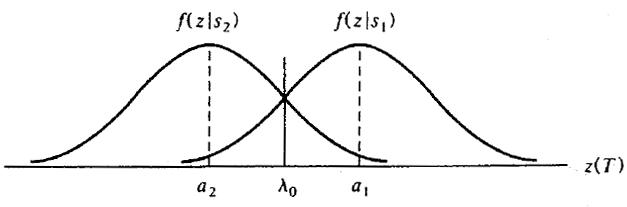
\includegraphics[width=8.5cm]{../NaT2/bilder/09_AWGN-PDF.png}
\end{minipage}
\begin{minipage}[c]{7cm}
	 $$ \lambda_0 = \dfrac{1}{2} (a_1 + a_2) + \dfrac{\sigma_{n_0}^2}{a_1 - a_2}
 \ln\dfrac{P(s_2)}{P(s_1)} $$ 
 	$$ \lambda_0 = \dfrac{a_1 + a_2}{2} \qquad (\text{gilt für: } P(s_2) = P(s_1) = \dfrac{1}{2})
 	$$
\end{minipage} 

Somit beträgt die Fehler-WSK: $ \qquad P_e = \textcolor{red}{P(H_2 | s_1)} P(s_1) + \textcolor{red}{P(H_1 | s_2)} = 
 P(s_1) \int\limits_{-\infty}^{\lambda_0} f(z|s_1) dz + P(s_2) \int\limits_{\lambda_0}^{\infty}
 f(z|s_2) dz$ \\
Mit ($P(s_2) = P(s_1) = \dfrac{1}{2}$) und ($\lambda_0 = \dfrac{a_1 + a_2}{2}$) gilt für ein
\textbf{NRZ-Signal}: $ \qquad P_e = Q \left(\dfrac{a_1 - a_2}{2 \sigma_{n_0}}\right) $



\subsection{Lineares Filter}
\skriptsubsubsection{Matched Filter}{229-9.4.A} \label{09_matched_filter}
	\textbf{Ziel: } Maximierung von $(a_1 - a_2)$ bei gleichzeitiger Minimierung
	von $n_0$. Mit $E_{s(t)}$ als Energie des Eingangssignals $s(t)$.
	%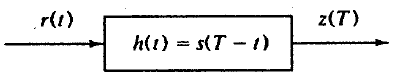
\includegraphics[width=4.5cm]{../NaT2/bilder/09_matched_filter.png}
 
	$$\text{SNR wird maximal bei} H \left( \omega \right) = S^* \left( \omega
	\right) \e^{-\jmath \omega T} \quad \IFT \quad h \left( t \right) = 
	\begin{cases} s(T-t) & 0 \leq t \leq T \\
	0 & sonst\end{cases} \qquad \text{wobei } \left(\dfrac{S}{N}\right)_{0_{max}} =
	\dfrac{2E_{s(t)}}{\eta}$$
 	

\skriptsubsubsection{Korrelator}{230-9.4.B} \label{09_korrelator}
Für den Sample Zeitpunkt ($t=T$) sind die Eigenschaften eines \textbf{Matched-Filter} und diejenigen eines
\textbf{Korrelators} \textbf{identisch}. Somit können beide für den selben Zweck eingesetzt werden.

$$ z(t) = r(t) \ast h(t) = \int_0^t r(\tau) h(t-\tau) d\tau \overbrace{=}^{h(t) =
h_{MatchedFilter}(t)} \int_0^t r(\tau) s[T - (t - \tau)] d\tau \overbrace{=}^{t = T} \int_0^T
r(\tau)s(\tau)$$

	\begin{center}
		\begin{minipage}[c]{4.5cm}
			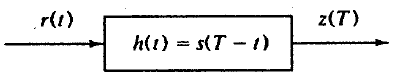
\includegraphics[width=4.5cm]{../NaT2/bilder/09_matched_filter.png}
		\end{minipage}
		\begin{minipage}[c]{2cm}		
			$$\Longleftrightarrow $$
		\end{minipage}
		\begin{minipage}[c]{4.5cm}
			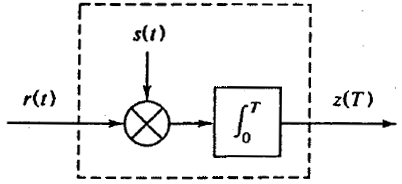
\includegraphics[width=4.5cm]{../NaT2/bilder/09_correlator.png}
		\end{minipage}
	\end{center}

\skriptsubsubsection{Unmatched RC-Filter}{238-Prob.9.9}
Hierbei wird an Stelle eines Matched Filters ein RC-Tiefpassfilter verwendet. \\
$$H(\omega) = \dfrac{1}{1 + j \omega R C}$$
% \qquad \dfrac{T}{RC} = 1.257 \qquad
%\left(\dfrac{S}{N}\right)_0_{max} = (0.815)\dfrac{2 A^2 T}{\eta}$$

\skriptsubsection{Fehlerwahrscheinlichkeit verschiedener binären
Übertragungen}{231-9.5}\label{09_binary_signals_error}
\small{$E_b$ bezeichnet die mittlere Signalenergie pro Bit.}\\
\renewcommand{\arraystretch}{2.5}
	\begin{tabular}{ p{6cm} p{2.5cm} p{9cm} }		
		\multicolumn{3}{l}{\textbf{Unipolar Baseband Signaling}} \\
		$ P_e = Q\left(\sqrt{\dfrac{A^2 T}{2 \eta}}\right) = Q\left(\sqrt{\dfrac{E_b}{\eta}}\right) $
		& $ E_b = \dfrac{A^2 T}{2} $
		& $ s_i(t) = \begin{cases}
		     s_1(t) = A & 0 \leq t \leq T \\       
		     s_2(t) = 0 & 0 \leq t \leq T
		   \end{cases}$ \\  

		\multicolumn{3}{l}{\textbf{Bipolar Baseband Signaling}} \\
		$ P_e = Q\left(\sqrt{\dfrac{2 A^2 T}{\eta}}\right) = Q\left(\sqrt{\dfrac{2 E_b}{\eta}}\right) $
		& $ E_b = A^2 T $
		& $ s_i(t) = \begin{cases}
 		     s_1(t) = +A & 0 \leq t \leq T \\       
 		     s_2(t) = -A & 0 \leq t \leq T
 		   \end{cases} $ \\

		\multicolumn{3}{l}{\textbf{Amplitude-Shift Keying}} \\
		$ P_e = Q\left(\sqrt{\dfrac{A^2 T}{4 \eta}}\right) = Q\left(\sqrt{\dfrac{E_b}{\eta}}\right) $
		& $ E_b = \dfrac{A^2 T}{4} $
		& $ s_i(t) = \begin{cases}
 		     s_1(t) = A \cos{\omega_c t} & 0 \leq t \leq T \\       
 		     s_2(t) = 0 & 0 \leq t \leq T
 		   \end{cases} $ \\

		\multicolumn{3}{l}{\textbf{Phase-Shift Keying}} \\
		$ P_e = Q\left(\sqrt{\dfrac{A^2 T}{\eta}}\right) = Q\left(\sqrt{\dfrac{2 E_b}{\eta}}\right)  $
		& $ E_b = \dfrac{A^2 T}{2} $
		& $ s_i(t) = \begin{cases}
 		     s_1(t) = A \cos{\omega_c t} & 0 \leq t \leq T \\       
 		     s_2(t) = A \cos{(\omega_c t + \pi)} = - A \cos{\omega_c t} & 0 \leq t \leq T
 		   \end{cases} $ \\

		\multicolumn{3}{l}{\textbf{Frequency-Shift Keying}} \\
		$ P_e = Q\left(\sqrt{\dfrac{A^2 T}{2 \eta}}\right) = Q\left(\sqrt{\dfrac{E_b}{\eta}}\right) $
		& $ E_b = \dfrac{A^2 T}{2} $
		& $ s_i(t) = \begin{cases}
 		     s_1(t) = A \cos{\omega_1 t} & 0 \leq t \leq T \\       
 		     s_2(t) = A \cos{\omega_2 t} & 0 \leq t \leq T
 		   \end{cases}$ \\

 	\end{tabular}
	\renewcommand{\arraystretch}{1}
\newpage
\section{Informationstheorie und Quellencodierung \schaum{245-10}}
\subsection{DMS - Discrete Memoryless Source}
Eine Informations\textbf{quelle} ist ein Objekt welches \textbf{Ereignise}, welche zufällig aus einer
WSK-Dichtefunktion ausgewählt werden, \textbf{generiert}. \\ 
Eine diskrete Quelle hat einen endlichen \textbf{Satz an Symbolen}, welcher auch \textbf{Alphabet}
genannt wird. Die Elemente dieses Satzes nennt man \textbf{Symbole} oder \textbf{Zeichen}. \\
Wird ein Symbol unabhängig vom Vorherigen generiert, so handelt es sich um eine DMS (diskrete
gedächtnisfreie Quelle). Eine solche wird mit folgenden Eigenschaften charakterisiert:
%\renewcommand{\parskip}{0}
\begin{itemize}\addtolength{\itemsep}{-0.3\baselineskip}
  \item Liste der Symbole - Alphabet
  \item Auftretenswahrscheinlichkeiten dieser Symbole - WSK-Dichtefunktion
  \item Symbolrate 
\end{itemize} 

\subsubsection{Informationsgehalt, Binary Unit, Entropie, Informationsrate \schaum{246-10.2-B.1,2,3}}
Mathematisch gesehen kann man sagen, je \textbf{unwahrscheinlicher} das \textbf{Eintreten} eines \textbf{spezifischen
Ereignisses} ist, desto \textbf{grösser} ist dessen \textbf{Informationsgehalt}.

\begin{multicols}{2}
\renewcommand{\arraystretch}{\arraystretchOriginal}
\begin{tabular}{|l|l|l|}
	\hline
	\textbf{Grösse}	& \textbf{Bezeichnung}	& \textbf{Einheit} \\ 
	\hline
	$I(x_i)$ 	& Informationsgehalt 	& b \\
	\hline
	$P(x_i)$	& Auftretens-WSK eines Symbols & \\
	\hline
	$H(x_i)$	& Entropie				& b/Symbol\\
	\hline
	$R$			& Informationsrate 		& b/s \\
	\hline
	$r$			& Symbolrate/Bitrate	& Symbole/s	 \\
	\hline
\end{tabular}

Der Informationsgehalt kann in folgenden Masseinheiten angegeben werden:
\[ [I(X)] = \begin{cases}
            	\text{bit (\emph{bi}nary uni\emph{t})} 
            		& \text{falls } base=2. \\
            	\text{hartley oder decit}
            		& \text{falls } base=10. \\
            	\text{nat (\emph{na}tural uni\emph{t})} 
            		& \text{falls } base=e
			\end{cases} 
\]
\textbf{Standardmässig} verwenden wir $base=2$, also bit oder gekürzt
\textbf{b}. Binary Unit ist ein Mass für den Informationsgehalt und sollte nicht mit dem Term ``bit'' (Binäres Zeichen) verwechselt
werden.
\end{multicols}

\begin{align*}
	I(x_i)	&= \log_{base} \frac{1}{P(x_i)} = - \log_{base} P(x_i) \\
	R		&= r H (X) \\
	H(X)	&= E[I(x_i)] = \sum\limits_{i=1}^m P(x_i) I(x_i) = - \sum\limits_{i=1}^m P(x_i) \log_2{P(x_i)} \qquad 0 \leq H(x) \leq \log_2(m) \\
	H(X|Y)	&=- \sum\limits_{j=1}^{n} \sum\limits_{i=1}^{m} P(x_i,y_j) log_2(P(x_i|y_j)) \\
	H(X,Y)	&=- \sum\limits_{j=1}^{n} \sum\limits_{i=1}^{m} P(x_i,y_j) log_2(P(x_i,y_j)) \\
	I(X;Y)	&=I(Y;X)=H(X)+H(Y)-H(X,Y)=H(X)-H(X|Y) 
\end{align*}


\subsection{DMC - Discrete Memoryless Channels \schaum{247-10.3}}
\begin{minipage}{9.5cm}
	\begin{center}
		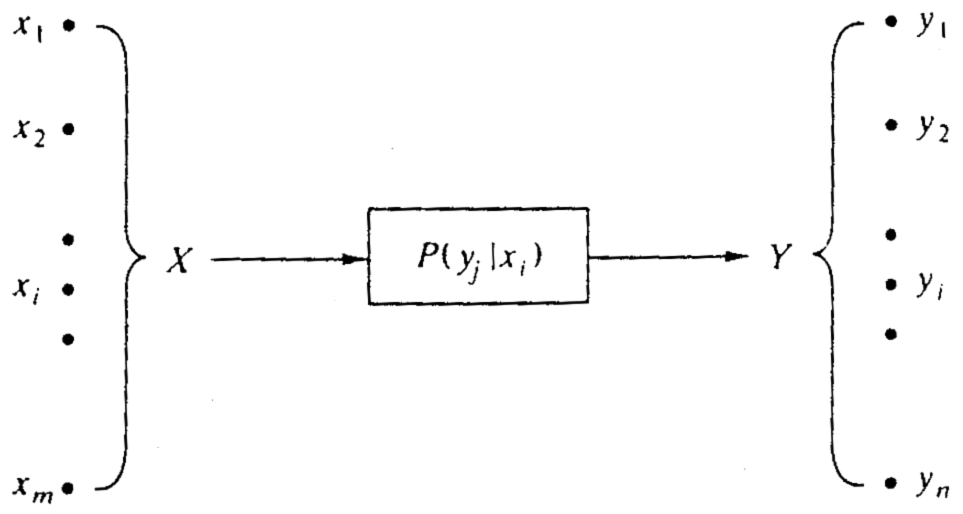
\includegraphics[width=7.5cm]{../NaT2/bilder/10_DMC.png}
	\end{center}
\end{minipage}
\begin{minipage}{8.5cm}
	Ein DMC (diskreter gedächtnisfreier Kanal) ist ein statistisches Modell mit Eingang $X$ und
	Ausgang $Y$. \\ \\
	Er besitzt \textbf{$m$ Eingänge} und \textbf{$n$ Ausgänge}. \\ \\
	Alle Auftretenswahrscheinlichkeiten $P(x_i)$ der einzelnen Eingangs-Symbole werden als gegeben
	betrachtet. \\
	Jeder Übertragungspfad ist durch die Kanal-Übertragungs-Wahrscheinlichkeiten (channel transition
	probabilities) $P(y_j | x_i)$ definiert.
\end{minipage}

\subsubsection{Darstellung in Matritzenform}
\begin{minipage}{9cm}
	\textbf{Kanalmatrix}
	$$ \boxed{[P(Y | X)] = \begin{bmatrix}
              P(y_1 | x_1) & P(y_2 | x_1) & \ldots & P(y_n | x_1) \\
              P(y_1 | x_2) & P(y_2 | x_2) & \ldots & P(y_n | x_2) \\
             . & . & . & . \\
              P(y_1 | x_m) & P(y_2 | x_m) & \ldots & P(y_n | x_m)
           \end{bmatrix}}$$ \\
	$ [P(Y)] = [P(y_1) \quad P(y_2) \quad \ldots \quad P(y_n)] = [P(X)] \cdot [P(Y|X)]$ \\
%	$ [P(Y)] =  \\
	$ [P(X)] = [P(x_1) \quad P(x_2) \quad \ldots \quad P(x_m)]$ \\ \\
	$\sum\limits_{j=1}^n P(y_j | x_i) = 1 (\forall i)$ \qquad $\sum$ jeder Zeile von $[P(Y|X)]=1$\\ \\
\end{minipage}
\begin{minipage}{9cm}
	\textbf{Verbundmatrix}
	\begin{center}$ \boxed{[P(Y,X)] = \begin{bmatrix}
              P(y_1, x_1) & P(y_2, x_1) & \ldots & P(y_n, x_1) \\
              P(y_1, x_2) & P(y_2, x_2) & \ldots & P(y_n, x_2) \\
             . & . & . & . \\
              P(y_1, x_m) & P(y_2, x_m) & \ldots & P(y_n, x_m)
           \end{bmatrix}}$
	\end{center}
	$  [P(Y,X)] =  \begin{bmatrix}
    	P(x_1) & 0 & \ldots & 0 \\
    	0 & P(x_2) & \ldots & 0 \\
    	. & . & . & . \\
    	0 & 0 & \ldots & P(x_m)
    \end{bmatrix} [P(Y|X)] $\\ 
	Elemente auf der Diagonale sollten den grössten Wert gegenüber anderen Elementen auf der Zeile
	besitzen. \\
	$\sum $ aller Elemente von $[P(Y,X)] = 1$
\end{minipage}

\subsubsection{Spezielle Kanäle \schaum{248-10.3.C}}
\textbf{Verlustfreier (lossless) Kanal} \\
\begin{minipage}{14cm}
	Auf jeder Spalte der Kanalmatrix gibt es jeweils nur ein  Element $\neq 0$. \\

	$$ [P(Y | X)] = \begin{bmatrix}
              \frac34 & \frac14 & 0 & 0 & 0 \\
              0 & 0 & \frac13 & \frac23 & 0 \\
              0 & 0 & 0 & 0 & 1
           \end{bmatrix}$$ \\
\end{minipage}
\begin{minipage}{5cm}
\begin{center}
	\adjustbox{width=5cm}{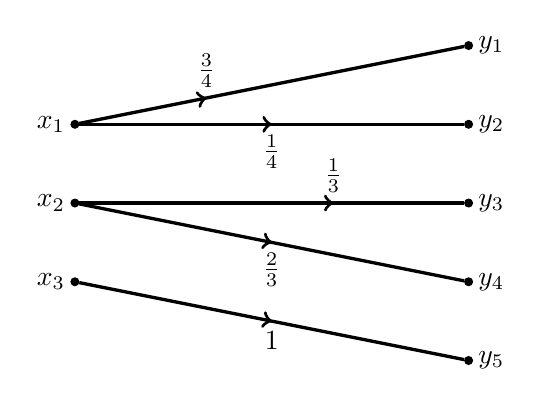
\begin{tikzpicture}
	\node (x1) at(0,0) [dot] {} (x1) node[anchor=east] {$x_1$};
	\node (x2) at(0,-1)[dot] {} (x2) node[anchor=east] {$x_2$};
	\node (x3) at(0,-2)[dot] {} (x3) node[anchor=east] {$x_3$};
	
	\node (y1) at(5,1) [dot] {} (y1) node[anchor=west] {$y_1$};
	\node (y2) at(5,0) [dot] {} (y2) node[anchor=west] {$y_2$};
	\node (y3) at(5,-1)[dot] {} (y3) node[anchor=west] {$y_3$};
	\node (y4) at(5,-2)[dot] {} (y4) node[anchor=west] {$y_4$};
	\node (y5) at(5,-3)[dot] {} (y5) node[anchor=west] {$y_5$};

	\draw[decorated onethird] (x1) -- node[pos=0.33, above] {$\frac{3}{4}$} (y1);
	\draw[decorated halfway]  (x1) -- node[pos=0.5, below] {$\frac{1}{4}$}  (y2);
	
	\draw[decorated twothird] (x2) -- node[pos=0.66, above] {$\frac{1}{3}$} (y3);
	\draw[decorated halfway] (x2) -- node[pos=0.5, below] {$\frac{2}{3}$}  (y4);
	
	\draw[decorated halfway] (x3) -- node[pos=0.5, below] {$1$} (y5);
\end{tikzpicture}}
\end{center}
\end{minipage}

\textbf{Deterministischer (deterministic) Kanal} \\
\begin{minipage}{14cm}
	Auf jeder Zeile der Kanalmatrix gibt es jeweils nur ein  Element $\neq 0$, welches $1$ sein
	muss.

	$$ [P(Y | X)] = \begin{bmatrix}
           		1 & 0 & 0 \\
           		1 & 0 & 0 \\
           		0 & 1 & 0 \\
           		0 & 1 & 0 \\
           		0 & 0 & 1
           \end{bmatrix}$$
\end{minipage}
\begin{minipage}{5cm}
\begin{center}
	\adjustbox{width=5cm}{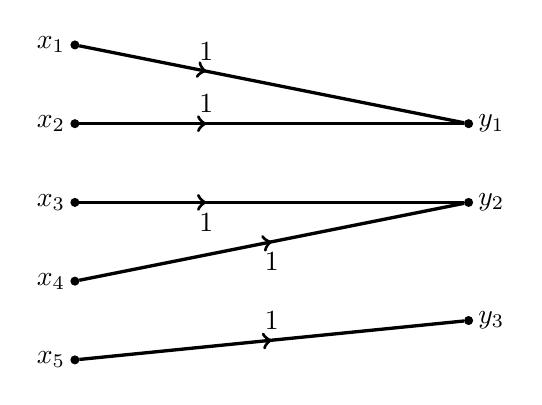
\begin{tikzpicture}
	\node (x1) at(0,0) [dot] {} (x1) node[anchor=east] {$x_1$};
	\node (x2) at(0,-1)[dot] {} (x2) node[anchor=east] {$x_2$};
	\node (x3) at(0,-2)[dot] {} (x3) node[anchor=east] {$x_3$};
	\node (x4) at(0,-3)[dot] {} (x4) node[anchor=east] {$x_4$};
	\node (x5) at(0,-4)[dot] {} (x5) node[anchor=east] {$x_5$};

	\node (y1) at(5,-1)  [dot] {} (y1) node[anchor=west] {$y_1$};
	\node (y2) at(5,-2)  [dot] {} (y2) node[anchor=west] {$y_2$};
	\node (y3) at(5,-3.5)[dot] {} (y3) node[anchor=west] {$y_3$};

	\draw[decorated onethird] (x1) -- node[pos=0.33, above] {$1$} (y1) ;
	\draw[decorated onethird] (x2) -- node[pos=0.33, above] {$1$} (y1);

	\draw[decorated onethird] (x3) -- node[pos=0.33, below] {$1$} (y2) ;
	\draw[decorated halfway] (x4) -- node[pos=0.5, below] {$1$} (y2);

	\draw[decorated halfway] (x5) -- node[pos=0.5, above] {$1$} (y3) ;
\end{tikzpicture}}
\end{center}
\end{minipage}

\textbf{Rauschfreier (noiseless) Kanal} \\
\begin{minipage}{14cm}
	Die Kanalmatrix entspricht der Einheitsmatrix.

	$$ [P(Y | X)] = \begin{bmatrix}
           		1 & 0 & \ldots & 0\\
           		0 & 1 & \ldots & 0\\
           		\vdots & \vdots & \vdots & \vdots \\
           		0 & 0 & \ldots & 1\\
           \end{bmatrix} = I$$ \\
\end{minipage}
\begin{minipage}{4cm}
\begin{center}
	\adjustbox{width=5cm}{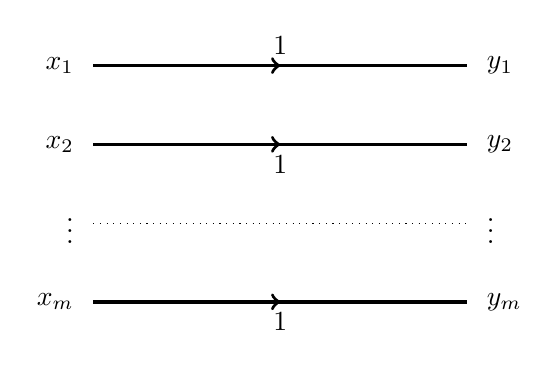
\begin{tikzpicture}
	\node (x1) at(0,0) {}   (x1) node[anchor=east] {$x_1$};
	\node (x2) at(0,-1) {}  (x2) node[anchor=east] {$x_2$};
	\node (xx) at (0,-2) {} (xx) node[anchor=east]{\vdots};
	\node (x3) at(0,-3) {}  (x3) node[anchor=east] {$x_m$};

	\node (y1) at(5,0) {}  (y1) node[anchor=west] {$y_1$};
	\node (y2) at(5,-1) {} (y2) node[anchor=west] {$y_2$};
	\node (yy) at(5,-2) {} (yy) node[anchor=west] {\vdots};
	\node (y3) at(5,-3) {} (y3) node[anchor=west] {$y_m$};

	\draw[decorated halfway] (x1) -- node[pos=0.5, above] {$1$} (y1);
	\draw[decorated halfway] (x2) -- node[pos=0.5, below] {$1$} (y2);
	\draw[dotted] (xx) -- (yy);
	\draw[decorated halfway] (x3) -- node[pos=0.5, below] {$1$} (y3);
\end{tikzpicture}}
\end{center}
\end{minipage}

\textbf{Binärer Symmetrischer (binary symmetrical) Kanal} \\
\begin{minipage}{14cm}

	$$ [P(Y | X)] = \begin{bmatrix}
           		1-p_e & p_e \\
           		p_e & 1-p_e
           \end{bmatrix} $$
\end{minipage}
\begin{minipage}{4cm}
\begin{center}
	\adjustbox{width=5cm}{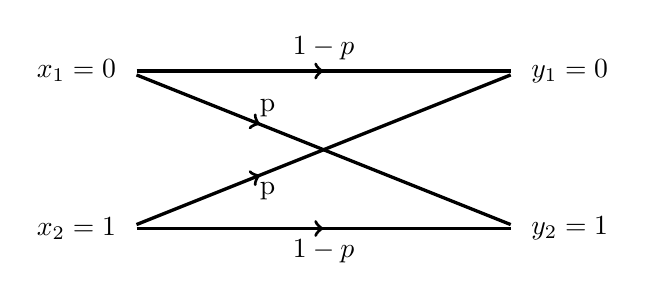
\begin{tikzpicture}
	\node (x1) at(0,0) {};
	\node (x2) at(0,-2) {};

	\node (y1) at(5,0) {};
	\node (y2) at(5,-2) {};

	\draw[decorated halfway] (x1) node[anchor=east] {$x_1=0$} -- node[pos=0.5, above] {$1-p$} (y1) node[anchor=west] {$y_1=0$};
	\draw[decorated onethird] (x1) -- node[pos=0.35, above] {p} (y2);

	\draw[decorated halfway] (x2) node[anchor=east] {$x_2=1$} -- node[pos=0.5, below] {$1-p$} (y2) node[anchor=west] {$y_2=1$};
	\draw[decorated onethird] (x2) -- node[pos=0.35, below] {p} (y1);

\end{tikzpicture}
}
\end{center}
\end{minipage}




% \subsection{Gegenseitige (mutual) Information \schaum{250-10.4}}
%  TODO \subsubsection{Bedingte Entropien}
%
%  TODO \subsubsection{Gegenseitige Information}
% \textbf{TODO}

\subsection{Kanalkapazität \schaum{251-10.5}}
\begin{minipage}[c]{8cm}
	$$ C_s = \max\limits_{\{ P(x_i) \}}{I (X; Y)} $$
	$$ C = r_b C_s $$
	$$ r_s H(X) \leq C$$
\end{minipage}
\begin{minipage}[c]{10cm}
	$C_s$ Kanalkapazität pro Symbol, $[C_s]$ = b/Symbol \\
	$C$ Kanalkapazität pro Sekunde, $[C]$ = b/s \\
	$r_s$ Symbolrate Quelle, $r_b$ Bitrate Kanal, $[r]$ = Symbol/s \\
	Bedingung für eine (theoretisch) fehlerfreie Übertragung
\end{minipage}

\subsubsection{Kanalkapazitätien spezieller Kanäle}

	\renewcommand{\arraystretch}{2}
	\begin{tabular}{| p{3.5cm} | p{7.5cm} | p{6.5cm} |}
		\hline  
    		\textbf{Verlustfrei}
    			& $ I(X; Y) = H(X) $
    			& $ C_s = \max\limits_{\{ P(x_i) \}}{H (X)} = \log_2 m $ \\
		\hline
    		\textbf{Deterministisch}
    			& $ I(X; Y) = H(Y) $
    			& $ C_s = \max\limits_{\{ P(x_i) \}}{H (Y)} = \log_2 n $ \\
		\hline
    		\textbf{Rauschfrei}
    			& $ I(X; Y) = H(Y) = H(X)$
    			& $ C_s = \log_2 n = \log_2 m$ \\
		\hline
    		\textbf{Binär Symmetrisch}
    			& $ I(X; Y) = H(Y) + p_e \log_2 p_e + (1-p_e) \log_2 (1-p_e)$
    			& $ C_s = 1 + p_e \log_2 p_e + (1-p_e) \log_2 (1-p_e)$ \\
		\hline
    		\textbf{AWGN}
    			& $ C = 2 B C_s = B \log_2 (1 + \left(\frac{S}{N}\right)_0)$ 
    			& $ C_s = \max{I(X; Y) = \frac{1}{2} \log_2 (1 + \left(\frac{S}{N}\right)_0)}$ \\
		\hline
 	\end{tabular}
	\renewcommand{\arraystretch}{1} \\ \\
Wobei $B$ der Bandbreite des Kanals entspricht. 
% \subsection{AWGN-Channel \schaum{252-10.6}}
% \textbf{TODO}

\subsection{Quellencodierung \schaum{253-10.7}}

\subsubsection{Code-Länge, -Effizienz, -Redundanz \schaum{253-10.7.A/B}}
Gilt für eine DMS mit endlicher Entropie.
\begin{multicols}{2}
	\abovedisplayskip=-15pt % Hack um den überflüssigen Whitespace zu entfernen.
	\begin{align*}
		L 		 &= \sum\limits_{i=1}^m P(x_i) n_i \\
		\eta	 &= \frac{H(x)}{L} = \frac{L_{min}}{L} \\
		\gamma_c &= 1 - \eta \\
		R(x)	 &= \gamma_q = H_{max} - H(x) = \log_2(m) - H(x) \\
				 &= \log_2(m) + \sum\limits_{i = 1}^m p(x_i) \cdot \log_2( p(x_i))
	\end{align*}
	
	\begin{tabular}{lll}
		$L$ 		& Durschnitt. Codewort-Länge & $[L]$ = Bits/Symbol \\
		$L_{min}$ 	& kleinstmölgliches L &  \\
		$P(x_i)$	& Auftretens-WSK des Symbols \\
		$n_i$ 		& Symbollänge & $[n_i] = $ Bits \\
		$m$ 		& Anzahl Symbole des Codes \\
		$\eta$ 		& Effizienz \\
		$\gamma_c$  & Redundanz des Codes & \\
		$\gamma_q$ 	& $= R(x)$ Redundanz der Quelle \\
		$H(X)$ 		& Entropie &  $[H(X)] = $ b/Symbol 
	\end{tabular}
\end{multicols}

\subsubsection{Klassifizierung von Codes \schaum{254-10.7.C}}
	\renewcommand{\arraystretch}{2}
	\begin{tabular}{| p{6cm} | p{12cm} |}
		\hline
    	\textbf{Bezeichnung} & \textbf{Eigenschaften}  \\
		\hline  
    	\begin{minipage}[c]{6cm}  
	    	\textbf{Fixed Lengh Code} \\
	    	feste Länge 
      	\end{minipage}
    	& \begin{minipage}[c]{12cm}    
	    		Alle Codewörter haben die gleiche Länge. \\
	    		Bsp.: ASCII-Code. 
      	\end{minipage}
    	\\
		\hline
    	\begin{minipage}[c]{6cm}    
    		\textbf{Variable Lengh Code} \\
    		variable Länge 
      	\end{minipage}
    	& \begin{minipage}[c]{12cm}    
    		Codewörter haben unterschiedliche Länge. \\
    		Bsp.: Shannon-Fano, Huffman und Morse Code. 
      	\end{minipage}
    	\\
		\hline
    	\begin{minipage}[c]{6cm}    
    		\textbf{Prefix-Free Code} \\
    		präfixfrei 
      	\end{minipage}
    	& \begin{minipage}[c]{12cm}    
    		Kein Codewort dient als Präfix (Vorsible) für ein anderes Codewort. \\
    		Bsp.: Shannon-Fano oder Huffman Code, aber nicht Morse-Code. 
      	\end{minipage}
    	\\
		\hline
    	\begin{minipage}[c]{6cm}    
    		\textbf{Uniquely Decodeable Code} \\
    		eindeutig decodierbar 
      	\end{minipage}
    	& \begin{minipage}[c]{12cm}    
    		Kette von Codewörtern kann eindeutig wieder in die ursrünglichen Symbolfolgen
    		zurückgewandelt werden. \\
    		Präfixfreie Codes sind eindeutig decodierbar. 
      	\end{minipage}
    	\\
		\hline
    	\begin{minipage}[c]{6cm}    
    		\textbf{Instantaneous Code} \\
    		sofort decodierbar 
      	\end{minipage}
    	& \begin{minipage}[c]{12cm}    
    		Liefert nach Empfang jedes einzelnen Codeworts sofort ein eindeutiges Symbol. \\
    		Jeder Instantaneous Code mit minimaler Codelänge ist optimaler Code. 
      	\end{minipage}
    	\\
		\hline
    	\begin{minipage}[c]{6cm}    
    		\textbf{Optimal Code}  
      	\end{minipage}
    	& \begin{minipage}[c]{12cm}    
    		$\eta = 1 = 100 \% $ 
      	\end{minipage}
    	\\
		
		\hline
 	\end{tabular}
	\renewcommand{\arraystretch}{1}

\subsubsection{Kraft'sche Ungleichung \schaum{255-10.7.D}}
Wenn diese Ungleichung erfüllt ist, besagt sie, dass ein \textbf{eindeutig} und \textbf{sofort
decodierbarer} Code gefunden werden kann. \\
Gegeben ist eine Quelle mit \textbf{Alphabet $x_i$} der \textbf{Länge $m$}, wobei jedem
\textbf{Symbol $x_i$} kein Codewort aber eine \textbf{Codelänge $n_i$} zugewiesen ist.
$$ K = \sum\limits_{i=1}^{m} 2 ^{-n_i} \leq 1$$ 
Die Kraft'sche Ungleichung hilft jedoch zum Auffinden dieses Codes nicht weiter.

\subsection{Entropie Codierung \schaum{255-10.8}}
\textbf{Ziel:} Durchschnittliche Codelänge an Entropie annähern $ \Rightarrow $ Wirkungsgrad
steigern.

\subsubsection{Shannon - Fanno Codierung \schaum{255-10.8.A}}
\begin{multicols}{2}
	\begin{tabular}{|c|c|c|c|c|c|l|}
		\hline
		$x_i$	& $P(x_i)$ 	& Step 1	& Step 2	& Step 3 	& Step 4 	& Code \\
		\hline
		$x_1$	& 0.30		& 0			& 0			& 			&			& 00 \\
		\cline{4-4}
		$x_2$	& 0.25		& 0			& 1			& 			& 			& 01 \\
		\cline{3-4}
		$x_3$	& 0.20		& 1			& 0			& 			& 			& 10 \\
		\cline{4-5}
		$x_4$	& 0.12		& 1			& 1			& 0			& 			& 110 \\
		\cline{5-6}
		$x_5$	& 0.08		& 1			& 1			& 1			& 0			& 1110 \\
		\cline{6-6}		
		$x_6$	& 0.05		& 1			& 1			& 1			& 1			& 1111 \\
		\hline 
	\end{tabular}
	
	\columnbreak
	
	\textbf{Vorgehen:}
	\begin{enumerate}
		\item Symbole mit \textbf{absteigender} Wahrscheinlichkeit anordnen.
		\item Trennung in \textbf{2 Teilmengen} mit möglichst gleicher WSK.
		\item \textbf{Obere} Teilmenge Symbol \textbf{0}, \textbf{unterer} Teilmenge Symbol \textbf{1}
		  zuordnen.
		\item Weiterhin unterteilen gemäss obigen Schritten, bis keine Teilung mehr möglich ist.
	\end{enumerate}
	
	\textbf{Eigenschaften:}
	\begin{itemize}
  		\item Präfix frei
  		\item letzter Teilungsschrit liefert immer gerade Anzahl Codewörter 
	\end{itemize}
\end{multicols}



\subsubsection{Huffman Codierung \schaum{256-10.8.B}}
\begin{multicols}{2}
  \adjustbox{width=0.95\linewidth, frame}{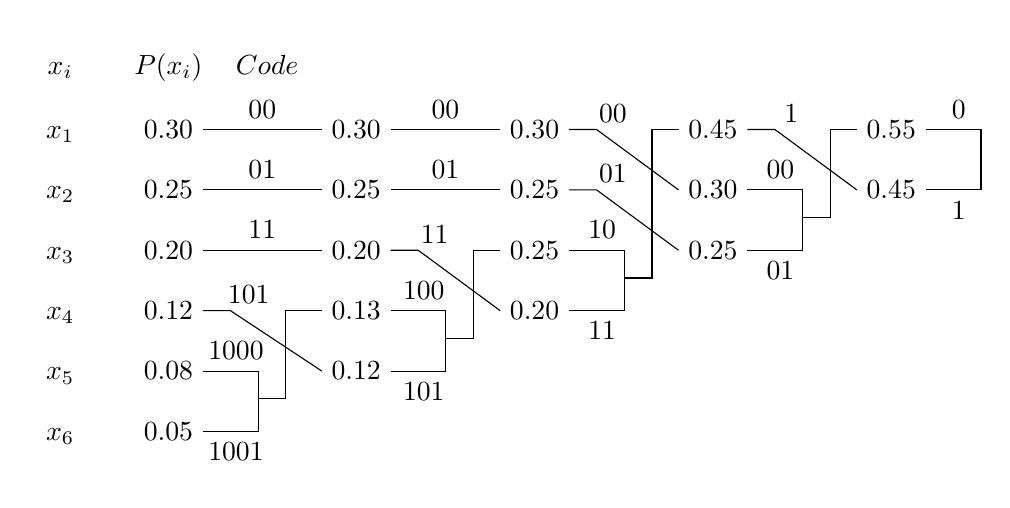
\begin{tikzpicture}[every node/.style={minimum height=2em}]
\matrix [matrix of math nodes](Mat)
{
x_i  &|[minimum width=1.5em]|& P(x_i) &|[minimum width=4em]| Code &       &|[minimum width=4em]|      &       &|[minimum width=4em]|  &   &|[minimum width=4em]|  &   &\\
x_1 &&0.30	&	& 0.30  &   &0.30   &   &0.45&  &0.55&\\
x_2 && 0.25	&	& 0.25  &   &0.25   &   &0.30&  &0.45&\\
x_3 && 0.20	&	& 0.20  &   &0.25   &   &0.25&  &   &\\
x_4 && 0.12	&	& 0.13   &   &0.20   &   &   &   &   &\\
x_5 && 0.08	&	& 0.12   &   &       &   &   &   &   &\\
x_6 && 0.05	&	&   &   &       &   &   &   &   &\\
};

\draw (Mat-2-3) -- (Mat-2-5) node[above=-0.1,midway]{00};
\draw (Mat-3-3) -- (Mat-3-5) node[above=-0.1,midway]{01};
\draw (Mat-4-3) -- (Mat-4-5) node[above=-0.1,midway]{11};
\draw (Mat-2-5) -- (Mat-2-7) node[above=-0.1,midway]{00};
\draw (Mat-3-5) -- (Mat-3-7) node[above=-0.1,midway]{01};

\draw(Mat-5-3.east) --++(1em,0) -- (Mat-6-5.west)node[above,pos=0.2]{101};
\draw(Mat-4-5.east) --++(1em,0) -- (Mat-5-7.west)node[above,pos=0.2]{11};
\draw(Mat-2-7.east) --++(1em,0) -- (Mat-3-9.west)node[above,pos=0.2]{00};
\draw(Mat-3-7.east) --++(1em,0) -- (Mat-4-9.west)node[above,pos=0.2]{01};
\draw(Mat-2-9.east) --++(1em,0) -- (Mat-3-11.west)node[above,pos=0.2]{1};

\draw (Mat-6-3.east)-|node[above=-0.1,pos=0.3]{1000}++(2em,-1em) coordinate(aa) --++(1em,0) |- (Mat-5-5.west);
\draw (Mat-7-3.east)-|node[below=-0.1,pos=0.3]{1001} (aa);

\draw (Mat-5-5.east)-|node[above=-0.1,pos=0.3]{100}++(2em,-1em) coordinate(bb) --++(1em,0) |- (Mat-4-7.west);
\draw (Mat-6-5.east)-|node[below=-0.1,pos=0.3]{101} (bb);

\draw (Mat-4-7.east)-|node[above=-0.1,pos=0.3]{10}++(2em,-1em) coordinate(cc) --++(1em,0) |- (Mat-2-9.west);
\draw (Mat-5-7.east)-|node[below=-0.1,pos=0.3]{11} (cc);

\draw (Mat-3-9.east)-|node[above=-0.1,pos=0.3]{00}++(2em,-1em) coordinate(dd) --++(1em,0) |- (Mat-2-11.west);
\draw (Mat-4-9.east)-|node[below=-0.1,pos=0.3]{01} (dd);

\draw (Mat-2-11.east)-|node[above=-0.1,pos=0.3]{0}++(2em,-1em) coordinate(ee);
\draw (Mat-3-11.east)-|node[below=-0.1,pos=0.3]{1} (ee);
\end{tikzpicture}}
  
  \columnbreak
  
  	\textbf{Vorgehen:}
  	\begin{enumerate}
	  \item Symbole mit \textbf{absteigender} Wahrscheinlichkeit anordnen.
	  \item \textbf{Unterste 2} Symbole als Gruppe zusammenfassen.
	  \item Beide Schritte wiederholen, bis nur noch zwei Gruppen vorliegen.
	  \item \textbf{Grössere} WSK \textbf{0}, \textbf{kleinere} WSK \textbf{1} zuordnen.
	  \item Reduktion rückgägngig machen und vorheriger Schritt für alle Teilschritte wiederholen.
	\end{enumerate}	
	
	\textbf{Eigenschaften:}
	\begin{itemize}
	  \item Maximale Effizienz
	  \item Keine reduntante Bits (vgl. Prüfung Aug. 2010)
	\end{itemize}
\end{multicols}

\newpage
\section{Kanalcodierung \skript{207-228}} 
\begin{center}
	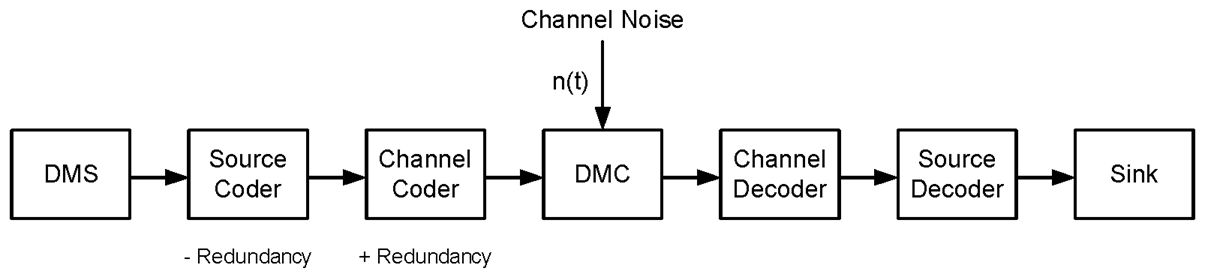
\includegraphics[width=11cm]{../NaT2/bilder/11_channel_coding_blockdiag.png}
\end{center}

Mit der Kanalcodierung können \textbf{Übertragungsfehler erkannt} und \textbf{beseitigt} werden.
Dies geschieht durch Beifügen geeigneter \textbf{Redundanz}. \\
Je nachdem wieviel Redundanz im Code vorhanden ist, handelt es sich um einen \textit{error-detecting
code} oder sogar um einen \textit{error-correcting code}.

\subsection{Kanalcodierungstheorem \skript{207}}
Gegeben seien DMS mit Entropie $H(X)$ und DMC mit Kanalkapazität $C_s$. 

\begin{itemize}
  	\item Für $H(X) < C_s$ kann mit geeigneter Kanalcodierung die \textbf{Fehlerrate} der
  	Übertragung \textbf{beliebig klein} gemacht werden. 
	\item Für $H(X) > C_s$ ist eine \textbf{fehlerfreie} Übertragung \textbf{nicht möglich}.
\end{itemize}
%Wenn man jedoch $n = \frac{H(x)}{C_s}$ Bits (binary digits) pro Symbol der Datenquelle bei
%geeigneter Codierung überträgt kann die Übertragung mit beliebig kleiner Fehlerrate erfolgen. \\ \\
Bitfehler in der Übertragung verunmöglichen einen zuverlässigen Informationsaustausch nicht,
sondern beschränken die nutzbare Übertragungsrate - je mehr Fehler desto mehr Übertragungsrate
wird für die Fehlerkorrektur benötigt. \\

\subsection{Blockcodes \skript{208-210}}
Hierbei werden aus (relativ kleinen) Datenblöcken mit \boldmath$k$ \textbf{Eingangssymbolen} Codes mit
je $n$ \unboldmath \textbf{Ausgangssymbolen} (mit $n > k$) generiert. Wobei jeder dieser Blöcke
separat codiert wird. Man spricht dann auch von einem $(n,k)$-Code. Beispielsweise handelt es
sich bei einer RS232-Übertragung mit 8 Daten- und 1 Paritätsbit um einen $(9,8)$-Code. \\
\hspace*{0.5cm} \parbox[c][1cm]{5cm}{\textbf{Coderate} $R_c = \frac{k}{n}$}\\
In unserem Fall (binär) kann ein Symbol zwei Zustände aufweisen. Diese Zustände sind in der binären
Menge ($K=\{0,1\}$) definiert.
Folgende mathematische Operatoren werden auf diese Menge angewendet:
\begin{itemize}
  \item Modulo-2-Addition: ``$\oplus$'' = logisches XOR $\quad\Rightarrow
  \quad(0,0)=0\;/\;(0,1)=1\;/\;(1,0)=1\;/\;(1,1)=0$
  \item Multiplikation: ``$\cdot$'' = logisches AND
\end{itemize}


\subsubsection{Lineare Blockcodes}
Ein Code gilt als linear, falls die Summe jeder beliebigen Codeworte ($\vec{a},\vec{b}$) wiederum auch ein
Codewort ($\vec{c}$) ist. 
$$\vec{a} = (a_1, a_2, \ldots, a_n) \quad \text{ und } \quad \vec{b} = (b_1, b_2, \ldots, b_n) \quad
\Longrightarrow \quad \vec{c} = \vec{a} \oplus \vec{b} = (a_1 \oplus b_1, a_2 \oplus b_2, \ldots, a_n \oplus b_n)$$

Wegen: $\quad \vec{a} \oplus \vec{a} = \vec{b} \oplus \vec{b} = 0 = (0,0,\ldots,0) \quad$, gilt \textbf{zwingend}, dass
zu jedem linearen Code der \textbf{Nullvektor} $\vec{0}$ gehört. Jeder Code der mit einer Generatormatrix
gebildet werden kann ist ein linearer Code.

\subsubsection{Hamming-Gewicht, (minimale) Hamming-Distanz}
\renewcommand{\arraystretch}{1.4}
\begin{tabular}[c]{ p{5.0cm}  p{5.0cm} p{9cm} }
	\textbf{Hamming-Distanz}:
	& $d(\vec{a},\vec{b}) = w(\vec{a} \oplus \vec{b})$
	& \textbf{Anzahl unterschiedliche Stellen} zweier Codeworte \\
	\textbf{Minimale Hamming-Distanz}\textcolor{red}{*}:
	& $d_{min} = \min[d(\vec{a},\vec{b})] \underbrace{= \min{[w(\vec{c})]}}_{\text{wenn lin. Code C}}$
	& \parbox[c]{9cm}{\textbf{Minimum} der Distanz aller mögl. Codewort-Paare\\
	Bei lin. Code: \textbf{Kleinstes} Hamming-Gewicht aller Codeworte} \\
	\textbf{Hamming-Gewicht}: 
	& $w(\vec{c}) = d(\vec{c},0)$
	& \textbf{Anzahl 1} eines Codeworts exkl. Nullvektor
\end{tabular}
\renewcommand{\arraystretch}{1} \\
\textcolor{red}{*}: Die Minimale Hamming-Distanz kann auch mittels der Paritätsprüfmatrix
\verweiskurz{paritycheckmatrix} berechnet werden.


\subsubsection{Fehlererkennungs- und Fehlerkorrektur-Möglichkeiten}
Durch die minimale Hamming-Distanz ist die Anzahl korrigierbarer und detektierbarer Fehler
gegeben. \\
\renewcommand{\arraystretch}{1.4}
\begin{tabular}[c]{ p{5.5cm}  p{13cm} }
	Anzahl \textbf{detektierbare} Fehler & $t_d = d_{min} - 1$ \\
	Anzahl \textbf{korrigierbare} Fehler & $t_c = \frac12 (d_{min} - 1) = \frac12 t_d$
\end{tabular}
\renewcommand{\arraystretch}{1} \\

\begin{minipage}{7.5cm}
	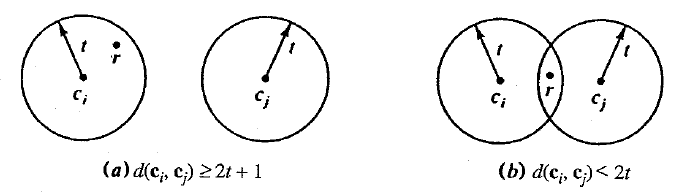
\includegraphics[width=7cm]{../NaT2/bilder/11_hamming_distance.png}
\end{minipage}
\begin{minipage}{11.5cm}
	Nebenan eine geometrische Veranschaulichung: Je mehr unterschiedliche Stellen (Hamming-Distanz)
	zwei Codeworte haben, desto weiter entfernt liegen die beiden Kreise - Abb. (a). Liegt deren
	Abstand (Hamming-Distanz) jedoch unter dem doppelten Radius ($< 2$), so kann der Decoder nicht mehr
	eindeutig feststellen, zu welchem ``Kreis'' das empfangene Zeichen gehört - Abb. (b).
\end{minipage} 

\subsection{Systematische Codes \skript{210-218}}
\begin{minipage}{5.5cm}
	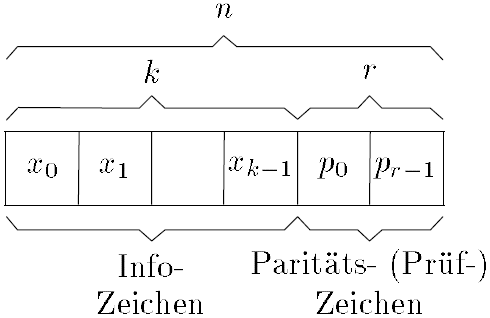
\includegraphics[width=5cm]{../NaT2/bilder/11_systematic_code.png}
	\centering geordnet-systematischer Code
\end{minipage}
\begin{minipage}{12.8cm}
	Ein Code gilt als systematisch, sobald alle \textbf{Datenbits} $d_i$ an irgendeiner Stelle des Codes $c_i$
	\textbf{unmodifiziert} vorkommen. Die nötigen Prüfzeichen werden meist am Ende
	der Datenbits angefügt und können, wenn gewünscht, ausgewertet werden.\\ Anwendungsbeispiele:
	\begin{itemize}
    	\item CRC (Cyclic Redundancy Check) bei MP3, JPEG, \ldots
    	\item Parity Check bei RS232
  	\end{itemize}	
	Die Coderate $R_C$ Ist das Verhältnis zwischen Codelänge und Nutzdaten: $\frac{k}{n}$
\end{minipage} 

\subsubsection{Generatormatrix G}
Mittels der \textbf{Generatormatrix} $G$ kann das jeweilige \textbf{Codewort} $\vec{c}$ aus dem \textbf{Datenwort} $\vec{d}$
generiert werden. Dimensionen: $\textcolor{blue}{[H\times B]}$
$$ \vec{c}\textcolor{blue}{_{[1 \times n]}} = \begin{bmatrix} c_1 & c_2 & \ldots & c_n \end{bmatrix} =
\vec{d}\textcolor{blue}{_{[1 \times k]}} \cdot G\textcolor{blue}{_{[k \times n]}} =
                \begin{bmatrix} d_1 & d_2 & \ldots & d_k \end{bmatrix} 
				\cdot \begin{bmatrix} 
					1 & 0 & \ldots & 0 & p_{11} & p_{21} & \ldots & p_{m1} \\              
					0 & 1 & \ldots & 0 & p_{12} & p_{22} & \ldots & p_{m2} \\
					\vdots & \vdots & \vdots & \vdots & \vdots & \vdots & \vdots & \vdots \\
					0 & 0 & \ldots & 1 & p_{1k} & p_{2k} & \ldots & p_{mk} \\
				\end{bmatrix} \overset{\textcolor{red}{*}}{=} \vec{d} \cdot [I\textcolor{blue}{_{[k \times k]}} \;
				P^T\textcolor{blue}{_{[k \times (n-k)]}}] $$ Bei $P^T$ handelt es sich um die transponierte
				Paritätsmatrix $P$, bei $I_k$ um die $[k \times k]$-Einheitsmatrix (\emph{I}dentität). \\
\textcolor{red}{*}: Das letzte Gleichheitszeichen gilt nur, falls
es sich um einen systematischen Code handelt. Ansonsten ist auch der linke Teil der Generatormatrix
nicht genau mit der Einheitsmatrix ``gefüllt''.

\subsubsection{Paritätsprüfmatrix H} \label{paritycheckmatrix}
Die Paritätsprüfmatrix $H$ dient zur \textbf{Erkennung von Übertragungsfehlern}. 
$$H\textcolor{blue}{_{[(n-k) \times n]}} = \begin{bmatrix}P & I_{n-k}\end{bmatrix} \Rightarrow
H^T\textcolor{blue}{_{[n \times (n-k)]}} =
\begin{bmatrix} P^T \\ I_{n-k}\end{bmatrix} 
\qquad \qquad 
G \cdot H^T = \begin{bmatrix}I_k & P^T\end{bmatrix} \cdot 
 \begin{bmatrix} P^T \\ I_{n-k}\end{bmatrix} = P^T \oplus P^T = 0
	\qquad \qquad
	\vec{c} \cdot H^T = \vec{d} \cdot G \cdot H^T = \vec{0}
	 $$
Die Multiplikation der Generatormatrix mit der transportierten Paritätsprüfmatrix ergibt eine 
$[k \times (n-k)]$-\textbf{Nullmatrix}. Somit ergibt die Multiplikation eines
\textbf{gültigen Codeworts} und der transportierten Paritätsprüfmatrix immer ein $[1
\times (n-k)]$-\textbf{Nullvektor}. \\
Die \textbf{minimale Hamming-Distanz} $d_{min}$ des Codes $C$ entspricht genau der minimal
nötigen Anzahl irgendwelcher Zeilen von $H^T$, sodass deren \textbf{Linearkombination Null} ergibt.


\subsubsection{Auswertung des Fehlersyndroms}
Das \textbf{Fehlersyndrom} $s$ erlaubt die Erkennung und eventuelle Korrektur von Übertragungsfehlern.
Angenommen das empfangene Codewort $c_r$ ist mit einem \textbf{Fehlermuster} $e$ versehen.
$$\vec{c}_r = \vec{c} \oplus \vec{e} \qquad \qquad \vec{s}\textcolor{blue}{_{[1 \times (n-k)]}} = \vec{c}_r \cdot H^T = \vec{c}
\cdot H^T \oplus \vec{e} \cdot H^T = \vec{e} \cdot H^T$$

Bei einem Einzelfehler entspricht das Fehlersyndrom $s$ gerade einer \textbf{Zeile von }
\boldmath$H^T$\unboldmath . Die \textbf{Zeilennummer} $i$ entspricht genau der \textbf{fehlerhaften
Position} im Code. Um den Code zu korrigieren wird die entsprechende Position invertiert.
$$ \vec{e} = \begin{bmatrix} \underbrace{0}_{1} & \ldots & 0 & \underbrace{1}_i & 0 & \ldots & 0\end{bmatrix} $$ 
Sind \textbf{alle} Zeilen von $H^T$ \textbf{unterschiedlich} entspricht dies \boldmath $d_{min}
\geq 3$ \unboldmath . 
Zugleich kann bei Einzelfehlern aus $s$ das \textbf{Fehlerbit} $e_i$ \textbf{eindeutig} bestimmt und das 
empfangene Codewort $c_r$ \textbf{korrigiert} werden. \\

\textbf{Hamming-Schranke}\\
\begin{minipage}{12cm}
	Ein $(n,k)$-Blockcode kann bis zu t Fehler korrigieren, falls $n$
	und $k$ die nebenstehende Ungleichung erfüllen. Diese Bedingung ist notwendig aber \textbf{nicht
	hinreichend}. Massgebend sind die Linearität und die minimale Hamming-Distanz. \\
	Gilt das Gleichheitszeichen, so handelt es sich um einen sog. \textbf{perfekten Code}. \\
	Einzelfehler korrigierende, perfekte Codes nennt man \textbf{Hamming-Codes}.
\end{minipage} 
\begin{minipage}{7cm}
	$$ \qquad 2^{n-k} \geq \sum\limits_{i=0}^{t} \binom{n}{i} \quad$$ \\
	$$ \text{mit} \quad \binom{n}{i} = \dfrac{n!}{(n-i)! i!} \quad \text{oder TR: \textbf{nCr(n,i)}}$$
\end{minipage}

\newpage

\subsection{Zyklische Blockcodes \skript{218-226}}
Coder und Decoder von gewissen \textbf{linearen Blockcodes} sind ab einem Umfang von $n \gg 1$ und
$k \gg 1$ sehr \textbf{aufwendig} zu realisieren. \\
\textbf{Abhilfe} schaffen die zyklischen Blockcodes - eine \textbf{Untergruppe} der linearen Blockcodes -
welche es erlauben mit einem \textbf{kleinen Hardwareaufwand} Coder und Decoder zu realisieren. 
$$ \text{1-fache: }\sigma(\vec{c}) = \vec{c}^{(1)} = (c_{n-1}, c_0, c_1, \ldots, c_{n-2}) \qquad 
 \text{2-fache }\sigma^2(\vec{c}) = \sigma\{\sigma(\vec{c})\}= \vec{c}^{(2)} = (c_{n-2}, c_{n-1}, c_0, \ldots, c_{n-3}) \qquad
 \text{n-fache }\sigma^n(\vec{c}) = \vec{c} $$
Wenn die \textbf{zyklische Verschiebung} $\sigma (c)$ eines Codeworts $\vec{c} = (c_0, c_1, \ldots,
c_{n-1})$ wiederum ein \textbf{gültiges Codewort} $\vec{c}$ ergibt, so handelt es sich bei dem Code um
einen linearen Blockcode.


\subsubsection{Code-Polynom c(x), Modulo-2-Polynom Arithmetik}
Zur mathematischen Behandlung werden zyklische Codes als Polynome dargestellt, wobei die
Koeffizienten $c_i$ jeweils der binären Menge $K=\{0,1\}$ angehören.
$$ \vec{c} = (c_0, c_1, c_2, \ldots,
c_{n-1}) \quad \Longleftrightarrow \quad c(x) = c_0 + c_1 x + c_2 x^2 + \ldots + c_{n-1} x^{n-1} 
\qquad \qquad \text{Bsp.: } \vec{c} = (1, 0, 0, 1, 1, 0) \quad \Longleftrightarrow \quad c(x) = 1 + x^3 +
x^4$$

\textit{Addition, Subtraktion, Multiplikation:} \\
Die Polynome können auf die \textbf{übliche} Weise \textbf{multipliziert} und \textbf{addiert} werden,
\textbf{ausser} bei \textbf{gleichem Exponenten} ergibt eine \textbf{Addition Null}.
Im binären Fall sind die Modulo-2-\textbf{Addition} und
-\textbf{Subtraktion identische} Operationen. 
$$ mod2(x^k + x^k) = 0 \qquad mod2(x^k - x^k) = 0 \qquad mod2(0 + x^k) = x^k \qquad mod2(0 - x^k) = x^k$$

\textit{Division:}\\
Die Modulo-2-Division stellt eine etwas \textbf{spezielle} Rechnung dar.
Eine Divison von \boldmath$f(x)$ durch $h(x)$ ergibt den Quotienten $q(x)$ mit Rest $r(x)$
\unboldmath . 
$$ \dfrac{f(x)}{h(x)} = q(x) + \dfrac{r(x)}{h(x)} \qquad \Longleftrightarrow \qquad \boxed{f(x) = q(x)
\cdot h(x) + r(x)}$$ 
Um $q(x)$ und $r(x)$ zu berechnen muss man die \textbf{übliche Polynomdivision} anwenden, \textbf{jedoch}
bei Addition und Subraktion zwischen den Koeffizienten Modulo-2-Addition anwenden. \\ 
Der \textbf{Modulo Operator} stellt eine vereinfachte Schreibweise dar, die jedoch teils auch
\textbf{verwirrend} sein kann.
$$ (1) \quad r(x) = f(x) \mod{h(x)} \qquad \qquad 
(2) \quad a(x) = b(x) \mod{h(x)} \qquad \qquad 
(3) \quad x^n = 1 \mod{(1 + x^n)}$$
Gleichung 1 bedeutet, dass $f(x)$ geteilt durch $h(x)$ den Rest $r(x)$ ergibt. \\
Gleichung 2 soll ausdrücken, dass beide Polynome $a(x), b(x)$ durch $h(x)$ dividiert den selben
Rest ergeben. \\
Gleichung 3 will sagen, dass (für ein beliebiges $n$) $x^n$ durch $(1 + x^n)$ geteilt, denn Rest
$1$ ergibt. \\
Somit ist das \textbf{Chaos} perfekt. Folgendes ist zu beachten, um Klarheit zu schaffen:\\
Generell steht der Modulo-Operator \textbf{immer} auf der \textbf{rechten Seite der Gleichung}. 
Das \textbf{Rest-Polynom} $r(x)$ ist immer dasjenige mit dem \textbf{kleinsten Grad
}($\PolyGrad[r \left( x \right)] < \PolyGrad[h \left(x \right)]$ und
$\PolyGrad[r \left(x \right) ] < \PolyGrad[f \left( x \right)]$).
\\

\textit{Zyklische Verschiebung} \\
Eine $i$-\textbf{fache zyklische Verschiebung} eines Polynoms erfolgt in drei Schritten:
$$ c^{(i)}(x) = c(x) x^i \mod{(1+x^n)}$$
\begin{enumerate}
  \item Multiplikation des Codepolynoms $c(x)$ mit $x^i$
  \item Division mit $(1+x^n)$
  \item Divisionsrest $r(x)$ entspricht gerade $c^{(i)}(x)$
\end{enumerate}

\subsubsection{Generator-Polynom g(x)}
Jeder $[n,k]$ zyklische Code kann mit Hilfe des Generator-Polynoms $g(x)$ (vom Grade $(n-k)$)
durch Multiplikation mit dem Daten-Polynom $d=d_0 + d_1x + \ldots + d_{k-1}x^{k-1}$ gebildet werden.
$$ g(x) = \textcolor{blue}{g_0} + g_1 x + g_2 x^2 + \ldots + \textcolor{blue}{g_{n-k}} x^{n-k}
\quad \text{mit (} \textcolor{blue}{g_{n-k} = g_0 = 1} \text{) } \qquad \Longrightarrow \qquad
c(x) = d(x) \cdot g(x)$$
Das Generatorpolynom wird durch \textbf{Modulo-2-Faktorzerlegung} (sehr kompliziert) gewonnen: 
$$ (x^n + 1) = q(x) \cdot \textcolor{purple}{g(x)} \qquad \qquad \text{Bsp.: } \quad (n=7,k=4) \quad
\Rightarrow \quad (x^7 + 1) = (x+1)\textcolor{purple}{(x^3+x+1)(x^3+x^2+1)}$$ Jedes Polynom der
Faktorzerlegung vom Grad ($n-k$) mit $g_{n-k} = g_0 = 1$ kann als Generatorpolynom verwendet
werden. Mittels \textbf{\matlab{cyclpoly(n,k,'all')}} können alle möglichen Generatorpolynome
erzeugt werden.
% einige generatormatritzen mittels matlab einfügen?!?

%\subsubsection{Paritätsprüf-Polynom h(x) \schaum{288-11.5.D}}

\subsubsection{Syndrom-Polynom s(x)}
\begin{minipage}{13.1cm}
Das Fehlersyndrom $s(x)$ (vom Grad ($n-k$)) dient zur \textbf{Ermittlung von Übertragungsfehlern}.
Enthält das empfangene Codewort $c_r(x)$ ein \textbf{Fehlermuster} $e(x)$, so entspricht der
Rest der Division (Decodierung) dem sog. Fehlersyndrom $s(x)$.
$$ c_r(x) = c(x) + e(x) \quad \qquad \text{Fehlersyndrom: } \boxed{s(x) = c_r(x) \quad \mod{g(x)}} $$
% $$ d(x) = \dfrac{c(x)}{g(x)} \Longrightarrow \dfrac{c_r(x)}{g(x)} = d(x) + \dfrac{s(x)}{g(x)}$$
$$ \text{Aus } c(x) = d(x)\cdot g(x) \text{ folgt } s(x) = e(x) \mod{g(x)}$$

	Die Fehlermuster $e(x)$ und die dazugehörigen Fehlersyndrome $s(x)$ werden in einer
\textbf{Tabelle} erfasst, sodass bei einem Syndrom $s(x)$ gerade auf das entsprechende Fehlermuster $e(x)$
geschlossen und dieses korrigiert werden kann.
\end{minipage} 
\begin{minipage}{0.3cm}
$\quad$
\end{minipage}
\begin{minipage}{7cm}
	\begin{tabular}{| p{1.8cm} | p{2.8cm} |}
  		\hline
  			Fehler $e(x)$ & Fehlersyndrom $s(x)$ $= e(x)  \mod{g(x)} $ \\
  		\hline
  			$1$	&	$1 \mod{g(x)}$ \\
  			$x$	&	$x \mod{g(x)}$ \\
  			$x^2$	&	$x^2 \mod{g(x)}$ \\
  			$\vdots$ & $\vdots$ \\
  			$1 + x$ &	$1+x \mod{g(x)}$ \\
  			$1 + x^2$ &	$1+x^2 \mod{g(x)}$ \\
  			$\vdots$ & $\vdots$  	\\		
  		\hline
  	\end{tabular}
\end{minipage}

Ist der \textbf{empfangene Code korrekt}, so ist das Fehlersyndrom \boldmath$s(x) =
0$\unboldmath.\\ \\
Für einen zyklischen Code mit minimaler Hamming-Distanz $d_{min}$ hat jedes
Fehlermuster mit Hamming-Gewicht $< \frac12 d_{min}$ ein ganz \textbf{charakteristisches, eindeutiges Fehlersyndrom}, welches nur vom Fehler $e(x)$
abhängig ist.

\subsubsection{Codierung - Multiplikation}
\begin{minipage}{9cm}
	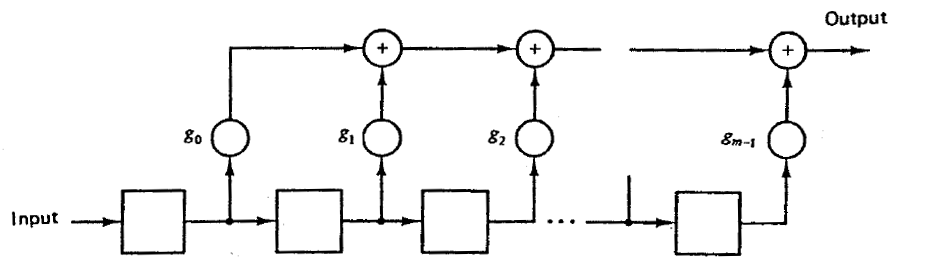
\includegraphics[width=9cm]{../NaT2/bilder/11_cyclic_coder_multiplication.png}
\end{minipage}
\begin{minipage}{9.5cm}
	Zur Codierung der Datenworte dient ein m-faches ($m = n-k$) \textbf{Schieberegister}. \\
	Das Datenwort muss mit \textbf{Zero-Padding} (konstante Länge, d.h. vorne mit 0 aufgefüllt) vorhanden sein.
	Zudem gilt in der nebenstehenden Form ``\textbf{LSB first}" ($d_0$) . Ist ``MSB first''($d_{k-1}$) gewünscht, so muss
	lediglich die Reihenfolge von $g_i$ getauscht werden.
\end{minipage}

\subsubsection{Decodierung - Division}
\begin{minipage}{9.4cm}
	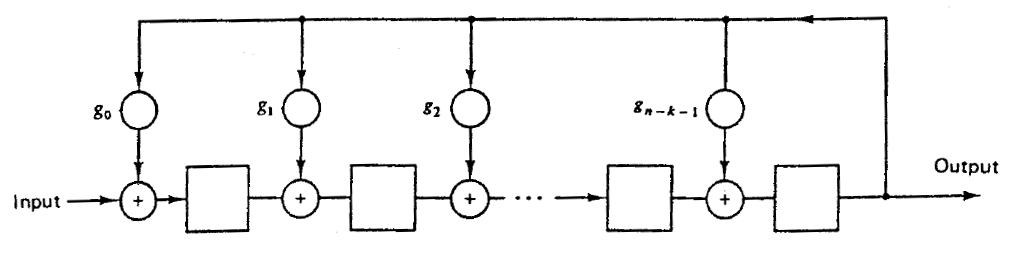
\includegraphics[width=9cm]{../NaT2/bilder/11_cyclic_decoder_division.png}
\end{minipage}
\begin{minipage}{9cm}
	Die Decodierung der Codeworte erfolgt durch ein (n-k-1)-faches \textbf{Feedback-Schieberegister}.\\
	Nach $n$-Taktzyklen entspricht der Ausgang dem Datenwort $d$ und der Inhalt des Schieberegisters
	dem Fehlersyndrom (Rest der Division). \\ 
	Das Codewort muss in der nebenstehenden Form mit \textbf{``MSB first''} ($c_{n-1}$) vorliegen.
\end{minipage}


\subsubsection{Realisierung eines systematischen Codes}
Ein zyklischer Blockcode kann immer in eine systematische Form gebracht werden, ohne dass die
Hamming-Distanz verändert wird oder die zyklischen Eigenschaften verloren gehen.
Die Matrix G eines nicht-systematischen zyklischen Codes kann durch die Zeilen $g(x), x\cdot g(x), \ldots, x^{k-1}\cdot g(x)$ gebildet werden. 
$\Rightarrow$ Durch Zeilenkombination (Additionen) kann G in eine systematische Form gebracht werden. Oft ist es üblich den systematischen Teil (Einheitsmatrix) im rechten Teil der Matrix G unterzubringen.\\
\hspace*{0.5cm}$ c(x) = p(x) + x^{n-k}\cdot d(x)$\\
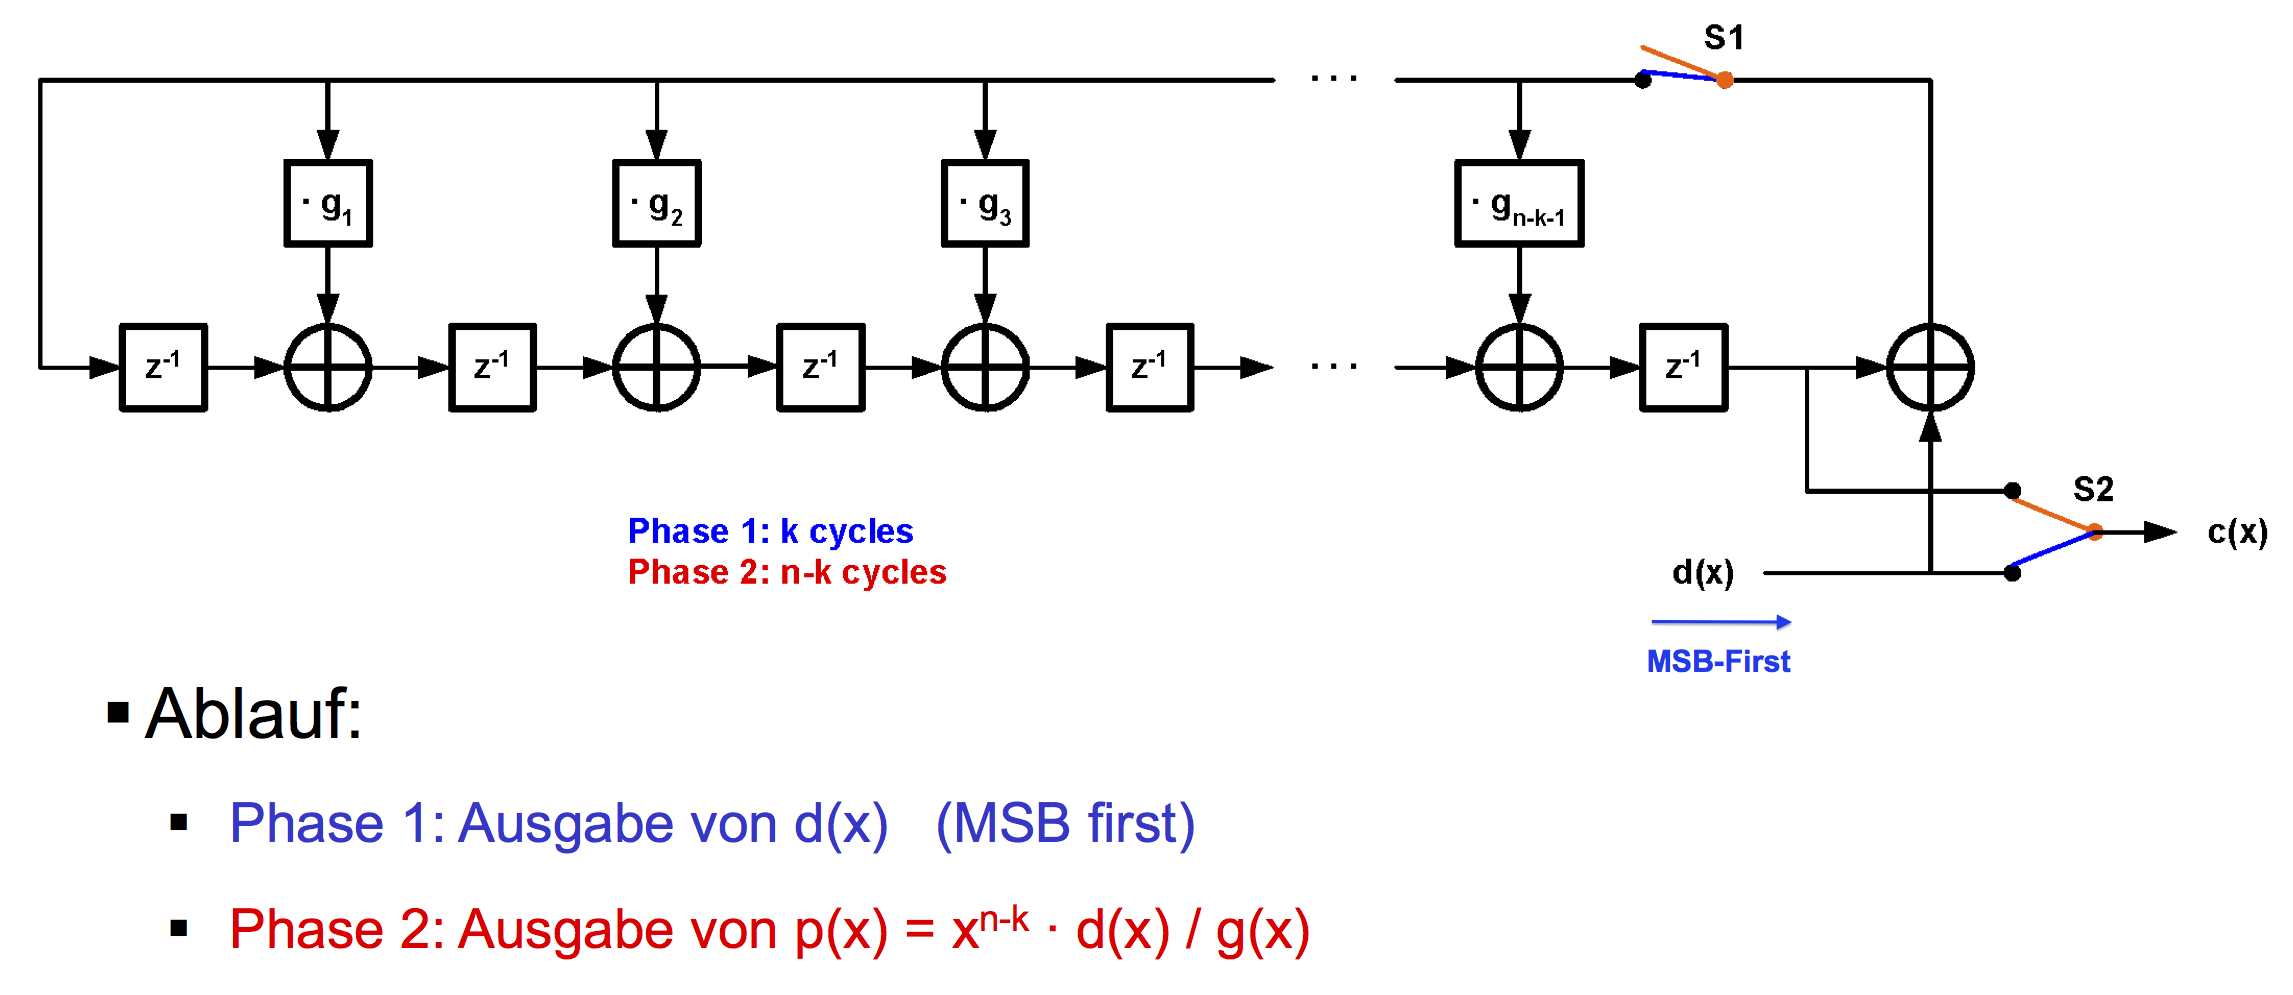
\includegraphics[width = 12cm]{./bilder/11_cyc_hw_imp_sys_code}

\subsection{Faltungscodes}
\textit{Nicht prüfungsrelevant!}\\ \\
Hierbei werden ganze Daten-Streams codiert. Der Code hängt hier nicht nur vom aktuellen Datenblock
ab, denn der Codierer bezieht auch noch einige vorgängige Blöcke in die Codierung mit ein.

\newpage
\section{Übungsverzeichnis}
\vspace{-\baselineskip}
\subsection{Wahrscheinlichkeitsrechnen und Zufallsvariablen}
	\begin{tabular}{|p{8cm}|p{2.5cm}|p{1.6cm}|p{4.9cm}|}
	\hline
	\textbf{Thema} & \textbf{Hausübung} & \textbf{Praktikum} & \textbf{Prüfung} \\ 
	\hline
	\hline
	Allgemein & 1.1-1.4 \newline 2.2-2.4 & & \\
%	\hline
%	MAP (maximale a posteriori) Entscheidungstheorie & 1.5 & 6.15 & \\
	\hline
	Zufallsvariable	& 2.1 & & 02.18: 5.1 \newline 08.16: 5.1 \\
%	\hline
%	Schütze - 2 dimensionale WSK-Verteilung & 2.5 & & \\
	\hline
	\end{tabular}
\subsection{Zufallsprozesse}
	\begin{tabular}{|p{8cm}|p{2.5cm}|p{1.6cm}|p{4.9cm}|}
	\hline
	\textbf{Thema} & \textbf{Hausübung} & \textbf{Praktikum} & \textbf{Prüfung} \\ 
	\hline
	\hline
	Wahrscheinlichkeitsfunktion & & & 08.18: 1.1 \newline 02.18: 1.1, 1.2 \newline 08.17: 1.1, 1.2 \newline 02.17: 1.1, 1.2 \newline 08.16: 1.1, 1.2 \newline 08.15: 2.1 \newline 08.13: 1.1, 1.2 \\
	\hline
	Leistung & & & 08.15: 2.2, 2.3\\
	\hline
	Autokorrelation	& & 3.5.1 \newline 5 (DTMF) & 08.18: 1.2 \newline 02.18: 1.3 \newline 08.17: 1.3 \newline 02.17: 1.3 \newline 08.16: 1.3 \newline 08.15: 2.4 \newline 08.13: 1.3 \\
	\hline
	Leistungsdichtespektrum & 4.1 \newline 5.1, 5.3 & 3.7.1 & 08.18: 1.3 \newline 02.18: 1.4 \newline 08.17: 1.4, 1.5 \newline 02.17: 1.4 \newline 08.16: 1.3, 5.3 \newline 08.15: 2.5 \newline 08.13: 1.4 \\
	\hline
	Stationarität & 3.1-3.3 & & 08.15: 5.2 \newline 08.13: 5.1\\
	\hline
	Ergodizität	 & 3.4 & & \\
	\hline
	Farbige Rauschsignale & & 3.4, 3.7.2 & 02.18: 5.2, 5.3 \newline 08.17: 5.4 \newline 02.17: 5.3 \newline 08.13: 5.2\\
	\hline
	\end{tabular}
\subsection{Rauschen in analogen Kommunikationssystemen}
	\begin{tabular}{|p{8cm}|p{2.5cm}|p{1.6cm}|p{4.9cm}|}
	\hline
	\textbf{Thema} & \textbf{Hausübung} & \textbf{Praktikum} & \textbf{Prüfung} \\ 
	\hline
	\hline
	Basisband & 6.1 & 4.3.2 & 08.18: 2.1, 2.2 \newline 08.17: 5.2, 5.3 \\
	\hline
	Rauschleistung (Equalizer) & 6.2 & 3.7.3 & 08.18: 5.1 \\
	\hline
	AM (DSB-SC), Synchronisation und SNR & 6.3, 6.6 & & 02.18: 2.1, 2.3, 2.5, 2.8, 2.9 \newline 08.15: 1.1 \\
	\hline
	AM (ordinary AM) & 6.4, 6.6 & 4.3.3 & 08.15: 1.2, 5.3 \\
	\hline
	FM/PM & 6.5, 6.6 & 4.3.4 & 08.18: 2.3-2.7 \newline 02.18: 2.2, 2.4, 2.6, 2.7, 2.10 \newline 08.16: 5.4 \newline 08.15: 1.3 \\
	\hline
	\end{tabular}
\subsection{Optimaler Detektor - Rauschen in digitalen Kommunikationssystemen}
	\begin{tabular}{|p{8cm}|p{2.5cm}|p{1.6cm}|p{4.9cm}|}
	\hline
	\textbf{Thema} & \textbf{Hausübung} & \textbf{Praktikum} & \textbf{Prüfung} \\ 
	\hline
	\hline
	Entscheidungsschwelle $\lambda$ & 7.1, 7.2 & & \\
	\hline
	Bitfehlerwahrscheinlichkeit & 7.3 & & 08.17: 2.2, 2.3 \newline 08.13: 2.2-2.5 \\
	\hline
	Matched Filter & 7.4 & & 08.17: 2.1 \newline 08.13: 2.1 \\
	\hline
	Unmatched Filter & 7.5 & & \\
	\hline
	\end{tabular}
\subsection{Informationstheorie und Quellencodierung}
	\begin{tabular}{|p{8cm}|p{2.5cm}|p{1.6cm}|p{4.9cm}|}
	\hline
	\textbf{Thema} & \textbf{Hausübung} & \textbf{Praktikum} & \textbf{Prüfung} \\ 
	\hline
	\hline
	Allgemein & & & 08.18: 3.7, 3.8, 5.4 \newline 02.18: 3.1-3.4, 5.4 \newline 08.17: 2.4-2.8, 3.3, 3.4, 3.6-3.9, 5.5 \newline 08.16: 2.1-2.5, 3.1, 3.2, 5.2, 5.6 \newline 08.15: 3.8-3.10, 5.4 \newline 08.13: 3.1, 3.2, 3.4-3.6, 5.6 \\
	\hline
	Information und Entropie & 8.1, 8.2 \newline 9.1, 9.2 & & 08.18: 3.1, 3.2, 3.5 \newline 02.18: 3.5, 3.6 \newline 08.17: 3.1, 3.2 \newline 02.17: 5.5 \newline 08.16: 3.5, 3.6 \newline 08.15: 3.5-3.7 \newline 08.13: 5.5 \\
	\hline
	Kanalmatrix/-diagramm & & & 08.18: 3.6 \newline 08.15: 3.3, 3.4\\
	\hline
	AWGN-Kanal & & & 08.18: 5.2, 5.3 \newline 08.17: 5.1 \newline 02.17: 5.4 \newline 08.15: 3.1, 3.2 \newline 08.13: 5.3 \\
	\hline
	Shannon Fano Codierung & 9.3-9.5 & & 08.13: 3.3 \\
	\hline
	Huffman Codierung & 9.4, 9.5 & 6 & 08.18: 3.3, 3.4 \newline 02.18: 3.7, 3.8 \newline 08.17: 3.5 \newline 08.16: 3.3, 3.4 \newline 08.15: 5.5 \newline 08.13: 3.7 \\
	\hline
	\end{tabular}
\subsection{Kanalcodierung}
	\begin{tabular}{|p{8cm}|p{2.5cm}|p{1.6cm}|p{4.9cm}|}
	\hline
	\textbf{Thema} & \textbf{Hausübung} & \textbf{Praktikum} & \textbf{Prüfung} \\ 
	\hline
	\hline
	Allgemein & & & 08.18: 5.5 \newline 08.13: 4.1, 4.2 \\
	\hline
	Blockcodes & 9.6 \newline 10.1, 10.2 \newline 11.1, 11.2 & 7.2 & 08.18: 4.1-4.5 \newline 02.18: 4.1-4.3, 4.5-4.8, 5.5 \newline 08.17: 4.1-4.3, 5.6 \newline 02.17: 4.4-4.8, 5.6 \newline 08.16: 5.5 \newline 08.15: 4.1-4.6, 5.6 \newline 08.13: 4.1, 4.2, 4.4-4.6, 4.8-4.11\\
	\hline
	Zyklische Codes & 11.3-11.5 & 7.3 & 08.18: 4.6-4.9, 5.6 \newline 02.18: 4.4, 4.9 \newline 08.17: 4.4-4.7 \newline 02.17: 4.1-4.3 \newline 08.16: 4.1-4.7 \newline 08.15: 4.2, 4.7 \newline 08.13: 4.3, 4.7\\
	\hline
	\end{tabular}
\subsection{Sonstiges}
	\begin{tabular}{|p{8cm}|p{2.5cm}|p{1.6cm}|p{4.9cm}|}
	\hline  
	\textbf{Thema} & \textbf{Hausübung} & \textbf{Praktikum} & \textbf{Prüfung} \\ 
	\hline
	\hline
	PLL - Phase Locked Loop	& & 1 & 02.17: 5.1 \\
	\hline
	8B/10B-Code & & 2 & 02.17: 5.2 \newline 08.15: 5.1 \newline 08.13: 5.4\\
	\hline
	\end{tabular}


\end{document}
